\chapter{Richtliniendemonstration}

Im Kapitel \ref{sec:analyse-der-aufgabenstellung} im Abschnitt ``\nameref{sec:architekturrichtlinien}'' ging das Projektteam auf die in der \nameref{sec:aufgabenstellung} vorgestellten Architekturrichtlinien und Prinzipien ein.

Als Ergebnis dieser Analyse entstand die unter Punkt \ref{sec:how-to-show-principles} vorgestellte, konsolidierte Liste mit Architekturrichtlinien.

Dieses Kapitel soll nun aufzeigen, wie und insbesondere wo eine jeweilige Architekturrichtlinie in der entwickelten Beispielapplikation demonstriert werden konnte.

Dabei wird zuerst verifiziert, ob die potentielle Demonstrationsstelle aus Tabelle \ref{fig:how-to-show-principles-matrix} wie erwartet umgesetzt werden konnte.
Anschliessend wird das konkret zur Richtlinie entstandene Beispiel näher analysiert und erklärt.

Am Ende dieses Kapitel wird bewertet, wie gut die jeweiligen Richtlinien an der Beispielapplikation demonstriert werden konnten.

\newpage
\section{Übersicht}

Folgende Tabelle bietet eine Übersicht über die Analyse aller in Abschnitt \ref{sec:how-to-show-principles} ``\nameref{sec:how-to-show-principles}'' definierten Richtlinien.

Die Spalte ``Resultat'' kann dabei die Ausprägungen ``Positiv'' oder ``Negativ'' haben.

\begin{figure}[H]
	\begin{table}[H]
		\tablestyle
		\tablealtcolored
		\begin{tabularx}{\textwidth}{l c c X}
			\tableheadcolor
				\tablehead Richtlinie &
				\tablehead\rotatebox{90}{Demonstriert\hspace{3mm}} &
				\tablehead\rotatebox{90}{Resultat} &
				\tablehead Bemerkung
				\tabularnewline
			\tablebody
				RP1	REST & \faOk & \faThumbsUp & \tabularnewline
				RP2 Application logic & & & \tabularnewline
				RP3 HTTP & \faOk & \faThumbsUp & \tabularnewline
				RP4 Link & \faOk & \faThumbsUp & \tabularnewline
				RP5 Non-Browser & \faOk & \faThumbsUp & \tabularnewline
				RP6 Should-Formats & & & \tabularnewline
				RP7 Auth & & & \tabularnewline
				RP8 Cookies & & & \tabularnewline
				RP9 Session & & & \tabularnewline
				RP10 Browser-Controls & & & \tabularnewline
				RP11 POSH & & & \tabularnewline
				RP12 Accessibility & & & \tabularnewline
				RP13 Progressive Enhancement & & & \tabularnewline
				RP14 Unobtrusive JavaScript & & & \tabularnewline
				RP15 No Duplication & & & \tabularnewline
				RP16 Know Structure & & & \tabularnewline
				RP17 Static Assets & \faOk & \faThumbsUp & \tabularnewline
				RP18 History API & \faOk & \faThumbsUp & \tabularnewline
				TP3 Eat your own API dog food & & & \tabularnewline
				TP4 Separate user identity and sign-up (...) & \faOk & \faThumbsUp & \tabularnewline
				TP7 Apply the Web instead of working around & & & \tabularnewline
				TP8 Automate everything or you will be hurt & \faOk & \faThumbsUp & \gls{CI}, Make\tabularnewline
			\tableend
		\end{tabularx}
	\end{table}
	\caption{Übersicht Architekturrichtlinienanalyse}
	\label{fig:how-to-show-principles-matrix}
\end{figure}



\newpage

%\section{RP1 REST}
\label{sec:principle-rp1-rest}

\gls{REST} beschreibt einen Architekturstil welcher grundlegende Auswirkungen auf die Strukturierung einer komplexen Client-Server Software hat und durch mehrere Randbedingungen gegeben ist:
\begin{itemize}
	\item Kommunikation zwischen Client und Server ist zustandslos
	\item HTTP wird als Grundlage verwendet
	\item \glspl{URI} sind Identifikatoren für Ressourcen auf dem Server
	\item Daten-Serialisierung (XML, JSON, etc.) ist nicht vorgegeben
\end{itemize}

Durch die Bedingung der Zustandlosigkeit wird durch Einsatz dieses Stils ermöglicht, skalierbare Schnittstellen zur Verfügung zu stellen.

Eine weitere Implementationstechnik von REST-APIs ist die Versionierung. Diese ermöglicht es Client und Server unabhängig voneinander weiter zu entwickeln.
Sobald die API eine neue Version erstellt und Rückwärtskompatibilität mit den alten Versionen garantiert, kann die Client-Software weiterentwickelt werden.

REST liegt HTTP zugrunde. Es werden explizit die sogenannten HTTP-Verben (GET, POST, PUT, DELETE etc.) verwendet um Ressourcen abzufragen oder zu manipulieren.
Durch den Einsatz des HTTP-Standards wird Caching auch direkt ermöglicht. Voraussetzung dafür ist, dass die Software die entsprechenden Caching-Headers in den Antworten sendet.

Damit spezifische Instanzen einer Ressourcen ansprechbar sind, ist die Verwendung korrekter und eindeutiger \glspl{URI} Pflicht. Jeder Objekt-Typ und jedes Objekt sollte eindeutig identifizierbar sein.

Der Datentyp mit welchem Objekte und Collections übertragen werden ist hingegen nicht definiert. Dem Software Entwickler ist die Serialisierung der Daten somit selber überlassen.
Vielfach wird heute jedoch \gls{JSON} eingesetzt, da es eine kompakte und doch gut lesbare Serialisierungsform ist.


\subsection*{Geplante Umsetzung}
Die Beispielapplikation \emph{Roomies} soll REST mit JSON als Datentyp für seine API verwenden.

Jede Ressource welche über die Website angefragt werden kann, soll auch über die REST-API verfügbar sein. Um den Sourcecode möglichst schlank halten zu können, soll auch intern die API verwendet werden.
Somit ist die API zwingend entkoppelt vom sonstigen Quelltext.

Eine Versionierung der API und das Caching der API-Zugriffe ist geplant.

\subsection*{Konkrete Umsetzung}
Die API der Beispielapplikation ist als separater Service-Layer implementiert worden. Auf diese wurd client- als auch serverseitig transparent zugegriffen.

Das Beispiel im Quelltext \ref{lst:restApiRoomies} zeigt zwei Definitionen einer solchen Route in der API.

\begin{lstlisting}[language=JavaScript, caption=Community API Definition \cite{communityApiDefinition}, label=lst:restApiRoomies, firstnumber=23, escapeinside={@}{@}]
var controller = require('./controller')
	, basicAuthentication = require('../policy/basicAuthentication')
	, authorizedForCommunity = require('../policy/authorizedForCommunity')
	, communityValidators = require('./validators')
	, utils = require('../utils')
	, modulePrefix = '/community';

module.exports = function initCommunityApi(api, apiPrefix) {
	var prefix = apiPrefix + modulePrefix;

	// GET /api/community/:id
	@\label{lst:restApiRoomies_get}@api.get(prefix + '/:id(\\d+)', [
		basicAuthentication
		, authorizedForCommunity
		, controller.getCommunityWithId]);

	// GET /api/community/:slug
	api.get(prefix + '/:slug', [
		basicAuthentication
		, authorizedForCommunity
		, controller.getCommunityWithSlug]);

	// POST /api/community
	@\label{lst:restApiRoomies_post}@api.post(prefix, [
		basicAuthentication
		, communityValidators.createCommunity
		, controller.createCommunity
	]);
	//...
};
\end{lstlisting}

Bei Zeile \autoref{lst:restApiRoomies_get} wird eine ``GET'' API für das Abfragen einer WG mit der \emph{ID} definiert. Wie man im definierten Array sieht, werden dabei mehrere Callbacks definiert, welche der Reihe nach aufgerufen werden und sicherstellen, dass jede Anfrage authentifiziert und authorisiert ist.

Zeile \autoref{lst:restApiRoomies_post} definiert eine ``POST'' Route um eine neue Community zu erstellen. Auch hier wird überprüft ob der Benutzer authentifiziert ist. Zudem wird auch ein Daten-Validator definiert, damit sichergestellt werden kann dass die Daten korrekt und ohne unerwünschte Zeichen sind.


Aus Zeitgründen wurde kein Caching und keine Versionierung implementiert.

Eine Versionierung wäre jedoch durch ein zusätzliches Präfix für die API-Route ohne Probleme lösbar.

Das selbe gilt für das Caching. Jedes Objekt in der Datenbank hat eine Spalte mit der Information, wann der Datensatz zuletzt modifiziert wurde. Durch diese Information kann generisch an einem Punkt ein Caching implementiert werden.

\subsection*{Diskussion}

REST ist ein immer wichtigerer Architekturstil und wird in dieser Form überall eingesetzt (siehe Twitter \cite{TwitterAPI}, Stripe \cite{StripeAPI}, etc.). Es definiert die wichtigsten Grundbedürfnisse und überlässt applikationsspezifische Entscheidungen dem Software Entwickler.

Seit einiger Zeit ist es immer wichtiger eine generische Schnittstelle auch für kleinere Websiten zu erstellen. Vielfach wird seit dem aufkommen von Smartphones nicht nur eine Website erstellt, sondern auch entsprechende Apps für Mobiltelefone.

Dadurch dass REST auch keine Serialisierungsform festlegt, ist es dem Entwickler der API möglich, verschiedene Datenformate zu unterstützen (siehe auch \ref{sec:principle-rp6-should-formats} ``\nameref{sec:principle-rp6-should-formats}''). Dies ermöglicht beispielsweise die Nutzung eines kompakten Datenformats für Mobiltelefone, damit die Datenrechnung nicht strapaziert wird.

Durch die relativ flexible REST-Definition mit einigen wenigen Randbedingungen tut sich aber auch ein wichtiger Diskussionspunkt auf: Mit welchem HTTP-Verb (POST oder PUT) werden Updates gehandhabt? Es gibt hier verschiedene Ansichten und die Diskussion ist bei Weitem nicht abgeschlossen. Eine gute Hilfestellung hierfür bietet ``Stack Overflow - HTTP PUT vs POST in REST'' \cite{StackoverflowPUTvsPOST}.

Abschliessend gibt das Projektteam folgenden Rat: Wenn es nötig ist eine flexible und generische API zu erstellen, ist REST eine sehr gute Lösung. Es erlaubt Entwicklern bestehendes Know-How über das Web wiederzuverwenden und die API wird durch die Zustandslosigkeit skalierbar.
\section{RP2 Application Logic}
\label{sec:principle-rp2-application-logic}

Die Logik einer Applikation kann in zwei Kategorien unterteilt werden:
\begin{enumerate}
	\item Businesslogik
	\item Präsentationslogik
\end{enumerate}

\subsection*{Businesslogik}
Die Businesslogik beinhaltet das eigentliche Herz der Applikation. Sie legt fest, welche Zustandsübergänge für Ressourcen möglich sind, welche Daten erlaubt sind und was bei API-Aufrufen ausgeführt wird.

Zur Businesslogik gehört laut den ``ROCA''-Autoren auch die \emph{logikbasierte Validierung}. Diese beinhaltet \cite{ObjektspektrumROCA} Funktionalität zur Überprüfung der Korrektheit der übertragenen Daten im Sinne der Businesslogik.

\subsection*{Präsentationslogik}
Bei jeder Aktion eines Benutzers müssen zwei Aktionen durchgeführt werden:
\begin{itemize}
	\item API-Aufrufe (lokal und remote)
	\item Darstellung der nächsten Ansicht
\end{itemize}
Welche API-Aufrufe gemacht werden und was die nächste Ansicht beinhaltet, bzw. welche Ansicht die nächste ist, kann als Präsentationslogik bezeichnet werden.

Zur Präsentationslogik gehört laut den ``ROCA''-Autoren die sogenannte \emph{datenbasierte Validierung} \cite{ObjektspektrumROCA}. Diese überprüft die Korrektheit der Daten aufgrund ihres gewünschten Datentyps (z.B. Telefonnummern auf formale Korrektheit etc.) und auch die Vollständigkeit der übertragenen Daten.
\\ \\
Damit eine Applikation ``RP2''-konform ist, darf jegliche vorangehend als Businesslogik beschriebene Logik nur auf dem Server implementiert werden. Die Duplizierung auf den Client würde dem \emph{``\gls{DRY}''}-Prinzip widersprechen und somit fundamentale Prinzipien des Software Engineerings verletzen.

\subsection*{Geplante Umsetzung}
Die Beispielapplikation soll trotz Code-Sharing ``RP2''-konform implementiert werden. Dies bedeutet, dass folgende Bedingungen beachtet werden sollen:
\begin{itemize}
	\item Businesslogik soll in der API implementiert sein
	\item Logikbasierte Validierung gehört zur Businesslogik und soll somit ebenfalls in der API umgesetzt werden
	\item Die Präsentationslogik wird einmal implementiert und sowohl auf dem Client als auch auf dem Server verwendet
	\item Die datenbasierte Validierung wird auf der API implementiert und falls möglich auch mit dem Client geteilt.
\end{itemize}

\subsection*{Konkrete Umsetzung}
Wie in Kapitel \ref{sec:sad} ``\nameref{sec:sad}'' gezeigt, wurde sowohl ein API- als auch ein Shared-Layer implementiert.

Die geplante Umsetzung konnte erfolgreich durchgeführt werden. Die API beinhaltet alle Businesslogik sowie die logikbasierte Validierung, während die ``Shared Codebase'' Präsentationslogik beinhaltet.

Die datenbasierte Validierung wurde aus Zeitgründen nur auf der API-Schicht implementiert und nicht mit dem Client geteilt. Dies wäre eine mögliche Weiterentwicklung.

\subsection*{Diskussion}
Ein Grundprinzip für Software Entwickler lautet \emph{``Never trust the client''} \cite{DefensiveProgramming}. Die Richtlinie \emph{RP2} lässt sich direkt auf dieses Prinzip anwenden.
Um sicherstellen zu können, dass jegliche übermittelte Daten eines Benutzers korrekt sind, müssen diese zwingend auf dem Server überprüft werden.

Diese Richtlinie ist für Client-Server Anwendungen wichtig. Was passiert aber, wenn Peer-to-Peer Anwendungen ohne zentralen Server implementiert werden sollen? Mit \mbox{\gls{WebRTC}} \cite{WebRTC} rückt dieses Thema vermehrt auch für Webapplikationen ins Zentrum der Aufmerksamkeit. Vermutlich kann dieses Prinzip nicht ohne weiteres auf solche Applikationen appliziert werden und bedarf darum weiterer Analysen von spezifischen Peer-to-Peer Patterns.
\\ \\
Im Projektteam ist man sich einig, dass diese Richtlinie für Client-Server Anwendungen umgesetzt werden muss. Falls man gewisse Codeteile sowohl auf dem Client als auch auf dem Server verwendet werden, kann es aber durchaus Sinn machen, schon auf dem Client diese Validierung zu machen. Dies dient aber vor allem der User Experience und darf niemals die Überprüfung auf dem Server ersetzen.

%\section{RP3 HTTP}
\label{sec:principle-rp3-http}

Das HTTP Prinzip von ROCA ist ähnlich wie Abschnitt \ref{sec:principle-rp1-rest} ``\nameref{sec:principle-rp1-rest}''.
Eine Applikation mit einer \gls{REST}-API ist die Grundvoraussetzung dafür, dass die Clientseite der Webapplikation mit dem Server \gls{RESTful} kommunizieren kann.

\subsection*{Geplante Umsetzung}
Die Kommunikation des Clients mit dem Server über \gls{REST} soll unter anderem über Backbone Models welche mittels den beiden Methoden ``save()'' und ``sync()'' bzw. ``fetch()'' (siehe \cite{BackboneSync}) mit dem Server kommunizieren.

Um normale HTML-Formulare \gls{RESTful} zu machen, soll ein Weg gefunden werden, mit dem nebst ``POST'' auch ``PUT'' und ``DELETE'' Abfragen ermöglicht werden.

\subsection*{Konkrete Umsetzung}
Die Umsetzung ist wie geplant ausgeführt worden. Als Beispiel zeigt Quelltext \ref{lst:roomiesCommunityModel} ein \emph{Barefoot.Model} \cite{barefootModel}, welches eine URL zur API definiert und über diese synchronisiert werden kann.

\begin{lstlisting}[language=JavaScript, caption=Community Model \cite{roomiesCommunityModel}, label=lst:roomiesCommunityModel]
/** Class: Models.Community
 * Community model as a subclass of <Barefoot.Model at
 * http://swissmanu.github.io/barefoot/docs/files/lib/model-js.html>
 */
var Barefoot = require('node-barefoot')()
	, Model = Barefoot.Model
	, CommunityModel = Model.extend({
		urlRoot: '/api/community'
		, idAttribute: 'id'
		, toString: function toString() {
			return 'CommunityModel';
		}
	});

module.exports = CommunityModel;
\end{lstlisting}

Um dieses Model mit Daten abzufüllen, kann wie in Quelltext \ref{lst:roomiesCommunitySync} gezeigt, eine Instanz geholt werden (Zeile \ref{lst:roomiesCommunitySync_dataStore}) und die ``fetch()''-Methode aufgerufen werden (Zeile \ref{lst:roomiesCommunitySync_fetch}).

\begin{lstlisting}[language=JavaScript, caption=Community Model Synchronisation \cite{roomiesCommunityJoinView}, label=lst:roomiesCommunitySync, firstnumber=10, escapeinside={@}{@}]
/** Function: initialize
 * Initializes the view
 */
, initialize: function initialize() {
	@\label{lst:roomiesCommunitySync_dataStore}@var community = this.options.dataStore.get('community');
	this.community = community;
}

/** Function: beforeRender
 * Before rendering it will fetch the community if not done yet.
 *
 * Parameters:
 *   (Promise.resolve) resolve - After successfully doing work, resolve
 *                               the promise.
 */
, beforeRender: function beforeRender(resolve) {
	/* jshint camelcase:false */
	var _super = this.constructor.__super__.beforeRender.bind(this)
		, resolver = function resolver() {
			_super(resolve);
		};

	if(!this.community.has('name')) {
		@\label{lst:roomiesCommunitySync_fetch}@this.community.fetch({
			success: resolver
			, error: resolver
		});
	} else {
		resolver();
	}
}
\end{lstlisting}

\subsubsection*{\gls{RESTful} Forms}
HTML-Formulare unterstützen nur zwei Arten von HTTP-Methoden, ``POST'' und ``GET'' \cite{FormMethodMDN}. Um eine Applikation \gls{RESTful} zu machen, sollten aber zumindest zusätzlich ``PUT'' und ``DELETE'' unterstützt werden.

Die Unterstützung dieser zusätzlichen Methoden erfordert eine Hilfskonstruktion:
\begin{itemize}
	\item Jedes Formular das nicht ``POST'' oder ``GET'' verwendet, erhält ein zusätzliches verstecktes Feld namens \emph{\_method} und dem Wert der gewünschten Methode
	\item Der Server interpretiert das Feld des vom Benutzer abgeschickten Formulars
	\item und ruft danach den entsprechenden Controller mit der entsprechenden Methode auf.
\end{itemize}

Quelltext \ref{lst:expressMethodOverride} zeigt die Anbindung der entsprechenden ``MethodOverride'' Middleware \cite{methodOverrideMiddleware} an eine Express-Applikation auf Zeile \ref{lst:expressMethodOverride_Override}.

\begin{lstlisting}[language=JavaScript, caption=HTTP Middleware \cite{roomiesHTTPMiddleware}, label=lst:expressMethodOverride, firstnumber=18, escapeinside={@}{@}]
/** Function: setupHttp
 * Adds described middlewares to the passed Express.JS application
 *
 * Parameters:
 *   (Object) app - Express.JS application
 *   (Object) config - Configuration
 */
function setupHttp(app, config) {
	var db = app.get('db');

	app.use(express.bodyParser());
	app.use(express.cookieParser());

	app.use(express.session({
		store: new SequelizeStore({
			db: db
		})
		, secret: config.sessionSecret
	}));

	@\label{lst:expressMethodOverride_Override}@app.use(express.methodOverride());
}

module.exports = setupHttp;
\end{lstlisting}

Als Beispiel zeigt Quelltext \ref{lst:taskCheckForm} das Formular für das abschliessen einer Aufgabe. Auf Zeile \ref{lst:taskCheckForm_MethodField} wird das entsprechende Feld definiert.

\begin{lstlisting}[language=JavaScript, caption=Formular mit verstecktem \emph{\_method} Feld \cite{taskCheckForm}, label=lst:taskCheckForm, firstnumber=6, escapeinside={@}{@}]
<form class="reset-style" action="/community/{{community.slug}}/tasks/{{id}}" data-task-id="{{id}}" method="post">
	@\label{lst:taskCheckForm_MethodField}@<input type="hidden" name="_method" value="put"/>

	<input type="hidden" name="name" value="{{name}}"/>
	<input type="hidden" name="reward" value="{{reward}}"/>
	<input type="hidden" name="dueDate" value="{{formatDate dueDate}}"/>
	<input type="hidden" name="fulfillorId" value="{{resident.id}}"/>
	<input type="hidden" name="fulfilledAt" value="{{formatDate now}}"/>

	<button type="submit" class="reset-style">
		<i class="icon-check-empty"></i>
	</button>
</form>
\end{lstlisting}

\subsection*{Diskussion}

``\nameref{sec:principle-rp3-http}'' ist eine Richtlinie, welche nach Auffassung des Projektteams nur hinsichtlich der Formulare bereichernd für den Konzeptkatalog ist. Die restliche \gls{REST} Thematik ist schon mit \nameref{sec:principle-rp1-rest} abgedeckt und sollte somit hinlänglich thematisiert worden sein.

Die Verwendung von ``PUT'', ``DELETE'' etc. für Formulare hat sowohl gute wie auch schlechte Seiten: Einerseits können die gleichen API-Routen (und somit der gleiche Code) wie für normale API-Aufrufe verwendet werden. Dafür ist allerdings ein relativ unschöner (aber doch relativ eleganter) Workaround zu verwenden.

Falls die eigene Applikation komplett mittels einer \gls{REST}-API aufgebaut wird ist diese Hilfskonstruktion sicher ein gehbarer Weg.
\section{RP4 Link}
\label{sec:principle-rp4-link}

\subsection*{Geplante Umsetzung}
Jede Seite innerhalb einer Web-Applikation muss mit einer eindeutigen URL adressierbar
sein.

Dies ist eines der ersten Paradigmas des Webs und auch eines der wichtigsten. In der Vergangenheit
ist es öfters vorgekommen, dass neuere Applikationen auf diesen ``Komfort'' verzichtet haben.
Heutzutage ist es aber u.a. dank der History API \cite{HistoryAPI} einiges
einfacher geworden, eindeutige URLs auch in JavaScript-lastigen Applikationen zu
verwenden.


\subsection*{Konkrete Umsetzung}
Weil die Beispielapplikation so oder so den REST \cite{REST} Prinzipien entspricht,
ist diese Richtlinie ein muss.

Jede URL entspricht einer eindeutigen Ressource und kann angesprochen werden.
Mithilfe der History API \cite{HistoryAPI} wird auch auf dem Browser die URL
geändert, obwohl u.U. nur ein AJAX-Request gemacht wird.

\subsection*{Diskussion}
Schon Tim Berners-Lee hat vor Jahren geschrieben: ``Cool URIs don't change'' \cite{CoolURIsTBL}.
Damit eine URL ``cool'' ist, muss sie zuerst mal vorhanden sein.

Auch aus einem weiteren Grund sind URLs nur dann ``cool'', wenn sie vorhanden sind
und niemals ändern: Mit den heuten Möglichkeiten des ``Sharing'' auf diversen Sozialen
Netzwerken muss es möglich sein, direkt auf die momentane Seite verlinken zu können.
%\section{RP5 Non Browser}
%\section{RP6 Should-Formats}
\label{sec:principle-rp6-should-formats}
Wie bereits der Name ROCA sagt, sollen Anwendungen ressourcen-orientiert sein. Damit diese Ressourcen auch in anderen Anwendungen als in einem Browser verwendet werden können, muss entweder das erzeugte HTML maschinenlesbar sein oder es müssen alternative Formate (wie z.B. JSON, XML usw.) verfügbar gemacht werden.

\subsection*{Geplante Umsetzung}
Im Abschnitt \ref{sec:principle-rp1-rest} \nameref{sec:principle-rp1-rest} wird darauf hingewiesen, dass eine REST API mit JSON als Datenformat verwendet werden soll.

\subsection*{Konkrete Umsetzung}
Abschnitt \ref{sec:principle-rp1-rest} \nameref{sec:principle-rp1-rest} zeigt, dass eine API umgesetzt wurde.
Die Schnittstelle liefert JSON als Ausgabeformat. Dies wird garantiert, indem ein Objekt an die Express.js Response \cite{ExpressjsResSend} zurückgeliefert wird und Express.js automatisch JavaScript Objekte in JSON umwandelt \cite{ExpressjsResponseJsonConverter}.

\begin{lstlisting}[language=JavaScript, caption=Community API getCommunityWithSlug \cite{roomiesCommunityApiExample}, label=lst:restApiCommunitySlug, firstnumber=333, escapeinside={@}{@}]
/** Function: getCommunityWithSlug
 * Looks up a community with a specific slug.
 *
 * Parameters:
 *   (Function) success - Callback on success. Will pass the community data as
 *                        first argument.
 *   (Function) error - Callback in case of an error
 *   (String) slug - The slug of the community to look for.
 */
function getCommunityWithSlug(success, error, slug) {
	debug('get community with slug');

	var communityDao = getCommunityDao.call(this);

	communityDao.find({ where: { slug: slug, enabled: true }})
		.success(function findResult(community) {
			if(!_.isNull(community)) {
				success(community.dataValues);
			} else {
				error(new errors.NotFoundError('Community with slug ' + slug +
					'does not exist.'));
			}
		})
		.error(function daoError(err) {
			error(err);
		});
}
\end{lstlisting}

Quelltext \ref{lst:restApiCommunitySlug} zeigt, wie das Community Objekt an den Success-Handler weitergegeben wird. Der Success-Handler ist von ``barefoot'' definiert und reicht den übergebenen Parameter an Express.js weiter. Express.js generiert daraus einen JSON String.

\subsection*{Diskussion}
Diese Richtlinie scheint auf den ersten Blick nicht sonderlich viel zu bringen. Wenn in einer Applikation sowieso nur JSON für API-Calls verwendet wird, wieso sollte dann z.B. zusätzlich XML unterstützt werden?

Die Richtlinie ist aber anders zu verstehen. Es soll zusätzlich zum generieren von HTML (welches aufgrund von \nameref{sec:principle-rp14-unobtrusive-javascript} ausdrücklich erforderlich ist) ein Ausgabeformat generieren, welches von Maschinen einfach lesbar ist (z.B. JSON oder XML).

Um die beiden Richtlinien \nameref{sec:principle-rp5-non-browser} und \nameref{sec:principle-rp14-unobtrusive-javascript} umsetzen zu können, muss auch diese Richtlinie umgesetzt werden. Ob JSON oder XML verwendet wird ist grundsätzlich egal und muss pro Applikation entschieden werden.

Das Projektteam kann diese Richtlinie uneingeschränkt empfehlen.
\section{RP7 Auth}
\label{sec:principle-rp7-auth}


Mit \emph{Basic Access Authentication} \cite{HTTPBasicAuth} steht seit Version 1.0 von \emph{HTTP} eine einfache Möglichkeit zur Verfügung, Ressourcen vom Zugriff Unbefugter zu schützen. Dank der frühen Integration in den HTTP Standard bedingten hohen Verbreitung, bringt der Verzicht auf Cookies, Session ID's oder Anmeldeseiten Eleganz durch Verwendung grundlegender Protokollfeatures.

Der Server kann durch Senden eines \emph{WWW-Authentication} Headers die Authentifizierung des Clients verlangen. Dieser wiederum sendet über den \emph{Authorization}-Header in seiner Antwort Benutzername und Passwort, welche mittels Base64 \cite{Base64} codiert sind.

Wird \emph{HTTP Basic Auth} in dieser Form verwendet, werden Benutzername und Passwort in Klartext über das Internet übertragen. Abhilfe schafft \emph{Digest Access Authentication}, wenn auch nur unbefriedigend. Hierbei werden die Identifizierungsmerkmale vor dem Übertragen mit einem Hashing-Algorithmus, bspw. MD5 maskiert. Der Server vergleicht dann den übertragenen Wert mit dem selbst berechneten Hash.

Insbesondere die Verwendung des MD5-Hashes gilt als unsicher \cite{MD5Broken}. Die Einfachheit von \emph{Basic Access Authentication} kann unter Verwendung des \emph{Secure Socket Layer} Protokolls \cite{SSL} problemlos beibehalten werden. Dabei wird die Kommunikation zwischen Client und Server in einen verschlüsselten \emph{\gls{SSL}}-Tunnel verpackt. Alle übertragenen Informationen sind so nicht mehr ohne weiteres von Dritten lesbar.

Um eine effiziente Sicherung von Ressourcen zu gewährleisten, schlägt \emph{RP7 Auth} die Verwendung des vorgestellten \emph{HTTP Basic Access Authentication over SSL} vor.


\subsection*{Geplante Umsetzung}

Die Umsetzung von \emph{HTTP Basic Authentication over SSL} ist nicht geplant. Im Bereich \emph{Security} und \emph{Authentication} soll der Fokus auf \nameref{sec:principle-tp4-seperate-user-identity} gelegt werden.

\subsection*{Konkrete Umsetzung}

Den Erwartungen entsprechend wurde das von \emph{RP7} vorgeschlagene \emph{HTTP Basic Authentication over SSL} nicht in der Beispielapplikation \emph{Roomies} implementiert.


\subsection*{Diskussion}

Die ROCA Richtlinie \emph{Auth} ergänzt die Forderungen von ``\nameref{sec:principle-rp5-non-browser}'': Die Kombination ermöglicht den browserfreien Zugriff auf geschützte REST-API-Ressourcen.

Für die Beispielapplikation \emph{Roomies} wurde aufgrund der umzusetzenden Anforderungen auf die Demonstration von \emph{RP7 Auth} verzichtet. Zwar bietet auch die in \ref{sec:principle-tp4-seperate-user-identity} ``\nameref{sec:principle-tp4-seperate-user-identity}'' vorgestellte Lösung eine sichere Variante, einen Benutzer für den Zugang zur Applikation zu authentisieren. Wie der Abschnitt \ref{sec:principle-rp5-non-browser} jedoch ausführlich beschreibt, kann dies nur mit einem Browser praktikabel funktionieren.

Nach Umsetzung der Beispielapplikation empfiehlt das Projektteam darum, sollte es mit den Aufwänden vereinbar sein, \emph{RP7 Auth} umzusetzen und die API via \emph{HTTP Basic Auth over SSL} zugänglich zu machen.
\section{RP8 Cookies}
\label{sec:principle-rp8-cookies}
Die ROCA Richtlinie RP8 legt fest, dass Cookies lediglich zur Authentifizierung oder zur statistischen Analyse (Tracking) eines Benutzers verwendet werden soll.

\subsection*{Geplante Umsetzung}
Die Beispielapplikation soll lediglich im Bereich der Anmeldung des Benutzers auf Cookies zurückgreifen.

\subsection*{Konkrete Umsetzung}
Das Geplante konnte mit Erfolg umgesetzt werden.
Um einem User eine Session zuzuweisen zu können verwendet Express.js \cite{Expressjs} die \gls{Middleware} ``\emph{connect-session}'' \cite{ConnectSession}.

Konnte ein Benutzer erfolgreich authentifiziert werden, sendet der Server dem Client ein Cookie mit einer eindeutigen Session-ID. Diese ID muss mit allen künftigen Requests mitgeschickt werden.

In der Beispielapplikation wird die Session-Middleware wie in Quelltext \ref{lst:connect-session-middleware} initialisiert:

\begin{lstlisting}[language=JavaScript, caption=Connect Session Middleware \cite{RoomiesMiddlewareHttp}, label=lst:connect-session-middleware, firstnumber=31]
app.use(express.session({
	store: new SequelizeStore({
		db: db
	})
	, secret: config.sessionSecret
}));
\end{lstlisting}

Der ``SequelizeStore'' \cite{SequelizeStore} übernimmt die Speicherung der Session-Daten innerhalb der Datenbank.

\subsection*{Diskussion}
Das Einbinden von mehr Informationen in Cookies hat mehrere Nachteile:
\begin{itemize}
	\item Sicherheit \\
		Wenn Benutzername und Passwort in ein Cookie gespeichert werden kann dies ohne Probleme von Drittpersonen mitgelesen werden. Falls HTTPS eingesetzt (auch wenn dies nur direkt im Browser geschieht) bildet dies ein nicht tragbares Risiko. \\
		Ausserdem ist es einem Benutzer möglich seine Cookies abzuändern. Dies könnte nur mithilfe von Validierung und dem Einsetzen eines \glspl{MAC} erkennbar gemacht werden.
	\item Datenmenge \\
		Cookies werden mit jeder Anfrage und jeder Antwort zwischen Client und Server mitgeschickt. Zwar ist die Grösse eines Cookies beschränkt, trotzdem wird die Datenmenge unnötig grösser.
\end{itemize}

Aus diesen Gründen sollte unbedingt darauf verzichtet werden, Cookies für andere Zwecke als für die wiederkehrende Authentifizierung über eine Session-ID oder für das Tracking zu verwenden. Für diese Zwecke eignen sich Sessions oder die Speicherung in die Datenbank besser.
%\section{RP9 Session}
\label{sec:principle-rp9-session}

Eine Session sollte ausschliesslich für simple Authentifizierungsinformationen verwendet werden. Dabei wird eine eindeutige Session-ID generiert, mit welcher der angemeldete Benutzer unmissverständlich erkennt werden kann. Dies reicht für die wiederholte Authentifizierung aus.

\subsection*{Geplante Umsetzung}
Der Session-Kontext soll nicht als Datenspeicher missbraucht werden. Aus diesem Grund soll dessen Verwendung auf die beschriebenen Authentisierungsinformationen beschränkt sein.

\subsection*{Konkrete Umsetzung}
Die für Benutzer-Authentifikation verwendete Bibliothek \emph{Passport.js} \cite{Passportjs} (siehe auch \ref{sec:principle-tp4-seperate-user-identity} ``\nameref{sec:principle-tp4-seperate-user-identity}'') speichert beim erstmaligen Anmelden eines Benutzers dessen Benutzerdaten serialisiert in die Session. Ab diesen Punkt hat \emph{Roomies} bis zum Löschen der Session Zugriff auf diese Informationen.

Um die User Experience zu steigern wurde entschieden, zusätzlich auch transiente Informationen im Session-Kontext zwischenzuspeichern. Konkret handelt es sich dabei um die Zielseite einer Weiterleitung, wie folgendes Beispiel verdeutlicht:

\begin{quotation}
Ein Benutzer von ``Roomies'' liebt es, sich mit den anderen Mitbewohner zu vergleichen. Deswegen besucht er oft die Rangliste. Auch einen Favorit hat er auf die Seite gesetzt, damit er direkt auf der Rangliste landet.

Ist der Benutzer noch nicht angemeldet und möchte die Rangliste besuchen wird er vom System aufgefordert sich anzumelden. Nach dem Anmeldevorgang wird ihm wie gewünscht jene Seite gezeigt.
\end{quotation}

Das Weiterleiten auf die Rangliste ist nur möglich, da der Server die \gls{URL} vor dem Anmelden in den Session-Kontext speichert, wie der Quelltext \ref{lst:router-set-redirecturl} zeigt.

\begin{lstlisting}[language=JavaScript, caption=Router - Autorisationskontrolle \cite{roomiesRouter}, label=lst:router-set-redirecturl, firstnumber=225]

/** Function: redirectIfNotAuthorized
 * If the client is not authorized it will redirect. Otherwise it returns
 * false to indicate that the calling method can continue work.
 */
, redirectIfNotAuthorized: function redirectIfNotAuthorized() {
	if(!this.isAuthorized()) {
		var req = this.apiAdapter.req;
		req.session.redirectUrl = req.originalUrl;
		this.navigate('', {trigger: true});
		return true;
	}
	return false;
}
\end{lstlisting}


\subsection*{Diskussion}
Wie in der konkreten Umsetzung beschrieben, kann diese Richtlinie nicht immer ohne Weiteres eingehalten werden.

Das Speichern vergleichsweise einfacher Informationen wie der Weiterleitungs-\gls{URL} ist aus Sicht des Projektteams vertretbar. Kritischer zeigt sich die Situation bei extensiver Nutzung des Kontexts. Wird zum Beispiel ein kompletter Warenkorb eines Webshops im Session-Kontext abgelegt, hat dies mehrere negative Auswirkungen: Zum einen gehen die Informationen verloren, sobald der Benutzer die Session beendet (Browser schliessen usw.), zum anderen skaliert diese Implementation bei vielen Sessions schlecht, da die Arbeitsspeicherauslastung linear zur Anzahl Sessions steigt. Für persistente, komplexere Session-Daten sollte entsprechend auf den Persistency-Layer zurückgegriffen werden.

Das Projektteam gibt entsprechend folgenden Ratschalg: Solange nur kleine, simple und temporäre Daten im Session-Kontext gespeichert werden, ist dies problemlos vertretbar. Es muss aber bei jeder Implementation genau überlegt werden, ob und welche Trade-Offs entstehen.
Weiter ist das Projektteam der Meinung, dass geschäftsprozess-kritische, transiente Informationen in keiner Situation im Session-Kontext abgelegt werden sollten.
%\section{RP10 Browser-Controls}
\label{sec:principle-rp10-browser-controls}
\begin{quotation}
Man befindet sich auf einem Online-Shop und sucht mit Hilfe der eingebauten Suche Zubehör für seine neu ergatterte Fotokamera. Das Suchresultat ist aber noch zu grob. Deshalb klickt man auf den Zurück-Knopf des Browsers um auf die Suche zurück zu gelangen. Aber was uns hier erwartet, ist nicht etwa das Suchformular, welches man erwartet hätte, sondern die Startseite.
\end{quotation}
Dies ist nicht etwa ein fiktives Beispiel, sondern ein reelles Szenario aus dem Online-Shop des Elektronikgrosshändlers Digitec \cite{Digitec}.

Das ROCA-Prinzip ``Browser-Controls'' will genau dieses unangenehme Erleben verhindern.

\subsection*{Geplante Umsetzung}

``Browser-Controls'' ist sehr eng mit dem Prinzip ``\nameref{sec:principle-rp4-link}'' verbunden. Indem jede Seite ihre eigene \gls{URI} hat und diese beim Navigieren in die ``History'' des Browsers eingefügt wird, funktionieren die Standardbedienelemente (Zurück, Vorwärts und Aktualisieren) eines Browsers erwartungsgemäss.

Dies soll auch in der Beispielanwendung ``Roomies'' der Fall sein. Jeder Seitenwechsel soll über den Webseitenverlauf im Browser nachvollziehbar sein und somit dem Benutzer erlauben, die eingebauten Funktionen des Browsers zu benutzen.

\subsection*{Konkrete Umsetzung}
Mit der Funktion ``Backbone.history.start()'' \cite{BackbonejsHistory} bietet Backbone.js eine Anbindung an die History API \cite{HistoryAPI} an und ermöglicht damit JavaScript Applikationen das dynamische Navigieren inklusive einer Aktualisierung der URL bei Seitenwechseln.

\begin{lstlisting}[language=JavaScript, caption=Activierung der History in Barefoot \cite{BarefootStartClient}, label=lst:barefootStartClientHistory, firstnumber=29]
// from modernizr, MIT | BSD
// http://modernizr.com/
var useHistory = !!(window.history && history.pushState);

Backbone.history.start({
	pushState: useHistory
	, hashChange: useHistory
	, silent: true
});
\end{lstlisting}

\subsection*{Diskussion}
-
%\section{RP11 POSH}
\label{sec:principle-rp11-posh}

``POSH'', ausgeschrieben ``Plain Old Semantic HTML'', bezeichnet das Erstellen von HTML-Seiten mithilfe von semantischen Elementen. \cite{SemanticHTML}

Semantisches HTML bietet den Vorteil, dass ``\glspl{SearchEngineSpider}'' die Seite besser verstehen, interpretieren und kategorisieren können. Wird eine Seite gut kategorisiert erscheint sie eher bei einer Suche in einer Suchmaschine wie Google oder Bing.

\subsection*{Geplante Umsetzung}
Die Seiten, respektiv deren HTML Markup, der Anwendung sollen eine klare und logische Struktur beinhalten.
Alle Seiten haben einen Titel, eine Überschrift und Inhalt.
Für Überschriften werden die Tags \emph{h1}, für die grösste und wichtigste Überschrift, bis \emph{h6} für die am wenig wichtigsten.
Tabellen sollen für tabellarische Daten verwendet werden und nicht etwa um die Seite zu strukturieren, wie es in der Vergangenheit oft angewendet wurde.

\subsection*{Konkrete Umsetzung}
Um die möglichen semantischen Inkorrektheiten zu reduzieren, wurde mit Templates gearbeitet. So können beispielsweise Menüs oder Fusszeilen definiert und wiederverwendet werden, ohne dass man diese bei jeder Benutzung neu schreiben muss. Dies geht sehr stark nach dem ``\gls{DRY}'' Prinzip. So werden Fehler verhindert, indem man sie gar nicht zu schreiben hat.

Im folgenden Beispiel-HTML sieht man einen kleinen Ausschnitt aus dem Haupttemplate von ``Roomies''. Man kann klar die Aufteilung der Seite erkennen. Oben beginnter der Header mit dem Menü, gefolgt von einem Platzhalter für allfälligen Fehler-, Warnungs- oder Informationsmeldungen. Die Hauptsektion mit der ID ``main''. Darin Befindet sich die ganzen Inhalte. Und zum Schluss die Fusszeile, in welcher sich der Abmelden-Link befindet.

\begin{lstlisting}[language=HTML, caption=Layout Definition \cite{roomiesHtmlSkeleton}, label=lst:layoutDefinition, firstnumber=27]
<body>
	<header id="menu"></header>
	<div id="flash-messages" class="row flash-messages"></div>
	<section id="main"></section>
	<footer id="footer"></footer>
</body>
\end{lstlisting}

\subsection*{Diskussion}

%\section{RP12 Accessibility}
\label{sec:principle-rp12-accessibility}
Aufbauend auf dem Prinzip ``\nameref{sec:principle-rp11-posh}'' besagt das Prinzip \emph{Accessibility}, dass alle Seiten für Hilfesoftware/-geräte wie \emph{Screen Reader} oder \emph{Braillezeile} zugänglich sein müssen.


``Barrierefreiheit schliesst sowohl Menschen mit und ohne Behinderungen als auch Benutzer mit technischen (Textbrowser oder PDA) oder altersbedingten Einschränkungen (Sehschwächen) ... ein.'' \cite{BarrierefreiesInternet}

\emph{RP12 Accessibility} beschränkt sich dabei auf Zugänglichkeit über Hilfeanwendungen. So wird die in der Definition erwähnte Problematik \emph{Farbblindheit} (richtige Farbenwahl etc.) oder die Navigation ohne Maus nicht abgedeckt.

\subsection*{Geplante Umsetzung}
Damit Hilfesoft- und Hilfehardware das User Interface der Beispielapplikation interpretieren kann, soll das HTML Markup, wie unter \ref{sec:principle-rp11-posh} ``\nameref{sec:principle-rp11-posh}'' erklärt, eine semantisch korrekte Struktur aufweisen.

\subsection*{Konkrete Umsetzung}

\emph{Roomies} verwendet, wo nötig, semantisch korrekte HTML-Elemente.

\subsection*{Diskussion}
In ``\nameref{sec:principle-rp11-posh}'' wird ausführlich über die Wichtigkeit eines barrierefreien Internets diskutiert. Das Prinzip \emph{RP12 Accessibility} strebt durch die notwendigen Vorkehrungen in die selbe Richtung, hat aber die Unterstützung gehandicapter Personen zum Ziel.

Leider gehört die Berücksichtigung von Farbenblindheit o.Ä. nicht zum Repertoire von \emph{RP12}. Für das Projektteam gehören aber auch diese Themen klar zum Aufgabenbereich der Richtlinie \emph{Accessibility}.

Das Projektteam schlägt darum die Ergänzung von \emph{RP12 Accessibility} um die erwähnten Punkte vor. Machen es die Anforderung nötig, empfiehlt das Projektteam die Umsetzung von \emph{RP12}.
%\section{RP13 Progressive Enhancement}
\label{sec:principle-rp13-progressive-enhancement}

\subsection*{Geplante Umsetzung}


\subsection*{Konkrete Umsetzung}


\subsection*{Diskussion}

%\section{RP14 Unobtrusive JavaScript}
\label{sec:principle-rp14-unobtrusive-javascript}

Aktuelle Webapplikationen können grob in zwei Kategorien eingeteilt werden:

\begin{figure}[H]
	\begin{table}[H]
		\tablestyle
		\tablealtcolored
		\begin{tabularx}{\textwidth}{l l X}
			\tableheadcolor
				\tablehead Kategorie &
				\tablehead Beispiel &
				\tablehead Erläuterung
				\tabularnewline
			\tablebody
				Statisch &
				\emph{GitHub} \cite{GitHub} &
				User Interface wird auf dem Server gerendert, JavaScript bringt lediglich dynamisch geladene Inhalte, Effekte oder zusätzliche ``optionale'' Features.
				\tabularnewline

				JavaScript Client &
				\emph{Google Drive} \cite{GoogleDrive} &
				User Interface wird komplett im Browser mittels JavaScript aufgebaut. Ohne JavaScript keine Funktionalität oder schlechtere User Experience.
				\tabularnewline
			\tableend
		\end{tabularx}
	\end{table}
	\caption{Kategorisierung aktueller Webapplikationen}
	\label{tab:current-webapplication-categories}
\end{figure}

Die Kategorie \emph{Statisch} zeichnet sich durch eine hohe Kompatibilität mit allen möglichen Internetbrowsern aus. Durch die Generierung des HTML Markups losgelöst vom schlussendlichen Zielclient, liegt die ganze Verantwortung, vom beschaffen anzuzeigender Daten bis hin zum zusammenstellen des HTML \gls{DOM}'s komplett bei der Serverkomponente.

Zwar kommt auch bei diesem Typus oftmals JavaScript zur Anwendung, meist beschränkt sich dessen Anwendung aber auf die Ergänzung des bereits statisch geladenen Inhaltes. So lädt \emph{Mila} \cite{Mila} beim Seitenwechsel, sofern JavaScript aktiviert, neuen Inhalt über einen \gls{AJAX} Request. Nach Erhalt des vorgerenderten HTML Markups aus der Antwort ersetzt es entsprechende Inhalte im aktuell angezeigten HTML \gls{DOM} des Browsers.

Als Programmiersprache auf dem Applikationsserver kommt hier oft Java, Python, PHP, Ruby o.Ä. zum Einsatz.

Beim puren \emph{JavaScript Client} liegt der Programmcode für das Rendern des User Interfaces mit all seinen Inhalten als JavaScript Quelltext vor. Nach erfolgreicher Übertragung zum Internetbrowser initiiert dieser die Erstellung der Applikationsoberfläche im HTML \gls{DOM} des Clients.

Sollen dynamische Informationen angezeigt werden, müssen diese über eine Serviceschnittstelle beim entsprechenden Anbieter angefragt werden (siehe bspw. Abschnitt \ref{sec:principle-rp1-rest} ``\nameref{sec:principle-rp1-rest}'').

Die Verlagerung des User Interface Quelltexts direkt in den Browser hat den Vorteil, dass UI Elemente effizienter verändert und aktualisiert werden können. Soll bspw. nur ein kleiner Teil der Benutzeroberfläche aktualisiert werden, kann dies gezielt und ohne Umweg über einen erneuten Request an den Server geschehen.

Durch diese Vereinfachung entfallen unnötige Wartezeiten zwischen Benutzereingabe und Systemreaktion. Dies resultiert wiederum in einer verbesserten User Experience.

Es ist bereits zu erahnen, dass diese Art von Webapplikation ohne JavaScript-Unterstützung im Browser nicht ausgeführt werden kann. Ein Beispiel hierfür liefert der \emph{Google Drive} \cite{GoogleDrive} Webclient. Wie in Abbildung \ref{fig:googleDriveNoJs} ersichtlich verweigert dieser ohne aktiviertes JavaScript die Funktion und zeigt ein leeres Standardlayout mit einer entsprechenden Meldung an.

\begin{figure}[H]
	\centering
	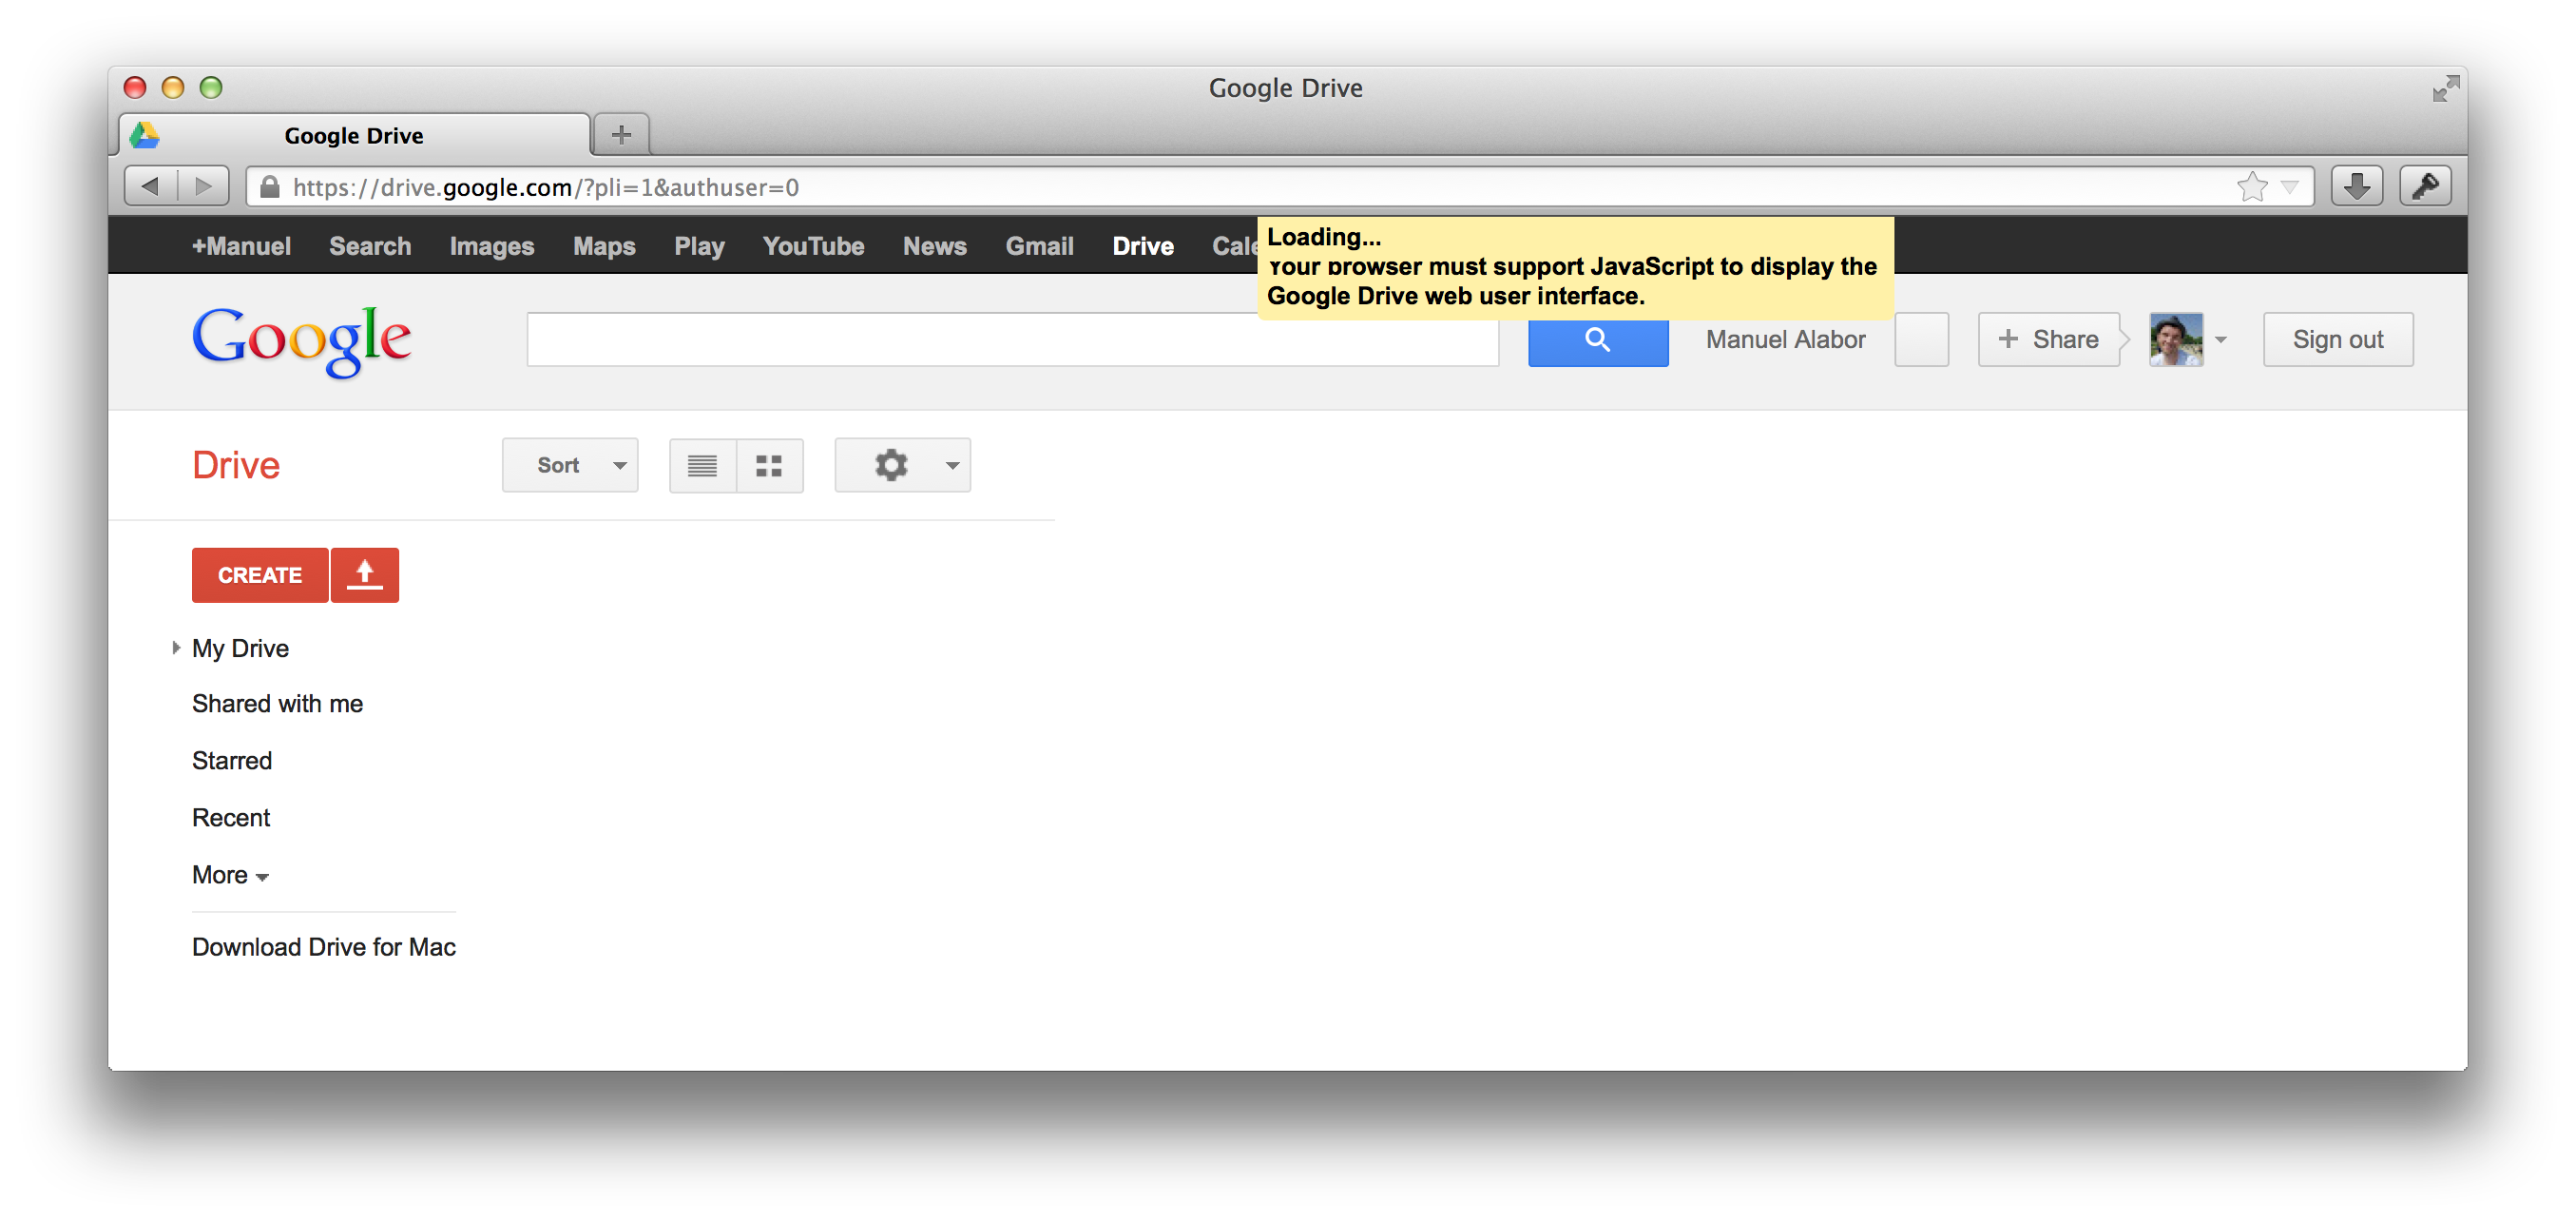
\includegraphics[width=12cm]{content/principle-demonstration/images/googledrive-nojs.png}
	\caption{\emph{Google Drive} in Firefox 21.0 mit deaktiviertem JavaScript}
	\label{fig:googleDriveNoJs}
\end{figure}

Die Richtlinie \emph{RP14 Unobtrusive JavaScript} aus dem ROCA Manifest verlangt, dass eine Webapplikation auch bei deaktiviertem JavaScript weiter funktionstüchtig bleibt. Soll JavaScript für ein modernes User Interface verwendet werden, muss gem. \emph{RP14} also eine Mischform aus den vorgestellten Applikationstypen verwendet werden.
\newline\newline
Bezieht man \emph{Unobtrusive Javascript} neben dem ``Wie und Wo'' User Interfaces gerendert werden auf die Thematik \emph{Codequalität}, gehört ein weiterer Aspekt zu diesem Bereich: Die Vermischung von HTML Markup und JavaScript Code soll unterbunden werden. Hierzu zeigt der Quelltext \ref{lst:badHtmlMarkupWithJavaScript} ein Beispiel, wie es unter keinen Umständen umgesetzt werden sollte.

\begin{lstlisting}[language=HTML, caption={Beispiel einer Vermischung von HTML Markup und JavaScript}, label={lst:badHtmlMarkupWithJavaScript}]
<a href="adresses.html" onClick="$('#progressIndicator').removeClass('hidden');showAddresses();return false;">
	Display Addresses
</a>
\end{lstlisting}

In den Quelltexten \ref{lst:goodHtmlMarkupWithoutJS} und \ref{lst:goodJSOutsideHtmlMarkup} ist ersichtlich, wie eine Separierung von JavaScript Logik und HTML Markup optimal implementiert wird.

\begin{lstlisting}[language=HTML, caption={Beispiel eines sauberen HTML Markups ohne JavaScript}, label={lst:goodHtmlMarkupWithoutJS}]
<a href="adresses.html" id="showAddresses">Display Addresses</a>
\end{lstlisting}

\begin{lstlisting}[language=JavaScript, caption={Beispiel Event-Handler in ausgelagerter JavaScript Datei}, label={lst:goodJSOutsideHtmlMarkup}]
$(function() {
	$('#showAddresses', showAddresses);

	function showAddresses(evt) {
		$('#progressIndicator').removeClass('hidden');
		// ... show addresses
		return false;
	}
});
\end{lstlisting}


\subsection*{Geplante Umsetzung}

Als Herausforderung hat das Projektteam geplant, die Beispielapplikation \emph{Roomies} als Mischung der vorgestellten Applikationstypen umzusetzen.

Grundsätzlich sollen Inhalte statisch auf der Backendkomponente gerendert werden. Hat der Benutzer in seinem Browser JavaScript aktiviert, ermöglicht entsprechender Programmcode die Umsetzung der im einleitenden Abschnitt vorgestellten Funktionalitäten eines vollwertigen \emph{JavaScript Clients}.

Zugriffe auf persistente Applikationsdaten sollen wie in \ref{sec:principle-rp1-rest} ``\nameref{sec:principle-rp1-rest}'' vorgeschlagen in ein entkoppeltes Serviceinterface gekapselt werden.

Um die Wartbarkeit der Codebasis zu optimieren, soll die Separierung von HTML Markup und JavaScript wie beschrieben strikt eingehalten werden.


\subsection*{Konkrete Umsetzung}

Während der Implementation der geplanten Lösung wurde sehr schnell klar, dass die entstehende Applikation zwar wie erwartet die gewünschte hybride Form aufweisen wird, aber keinesfalls mit der ROCA Richtlinie \emph{\nameref{sec:principle-rp15-no-duplication}} vereinbar sein wird.

Es hätten viele Codefragmente wie die View-Templates (Beispiel siehe Quelltext \ref{lst:reusableHandlebarsViewTemplate}) dank der durchgängigen Verwendung von JavaScript auch im Frontend wiederverwendet werden können. Andere, logikintensivere Komponenten wie die Controller zur Steuerung der eigentlichen User Interface Funktionalitäten (Event-Handling, Datenzugriffe etc.) hätten doppelt implementiert werden müssen.

\begin{lstlisting}[language=JavaScript, firstnumber=31, caption={Ausschnitt aus dem \emph{Handlebars} \cite{Handlebars} Template zur Darstellung von Benutzerinformation in der Menüleiste von \emph{Roomies} \cite{roomiesMenuTemplate}}, label={lst:reusableHandlebarsViewTemplate}]
{{#if user}}
<ul class="right">
	<li class="account">
		<a href="/resident/{{user.facebookId}}/profile">
			<span class="item-label">{{user.name}}</span>
			<img class="avatar small" src="//graph.facebook.com/{{user.facebookId}}/picture" />
		</a>
	</li>
</ul>
{{/if}}
\end{lstlisting}

Um diesem Umstand gegensteuern zu können teilte sich das Projektteam nach der ersten Entwicklungsiteration in zwei Gruppen:

\begin{itemize}
	\item Zwei Mitglieder arbeiteten weiter an der Umsetzung der geplanten Use Cases
	\item Ein Mitglied fokussierte sich auf die Entwicklung einer Möglichkeit, identischen Applikationscode sowohl in der Backend-Komponente für statisches Rendering als auch direkt im Browser als JavaScript Client verwenden zu können.
\end{itemize}

Aus diesem Prozess entstand das eigenständige Framework \emph{barefoot} \cite{Barefoot}. Es setzt auf der verbreiteten Bibliothek \emph{Backbone.js} \cite{Backbonejs} auf und ermöglicht die Verwendung einer einzigen, einheitlichen Codebasis für JavaScript-basierte Webapplikationen (siehe dazu auch Kapitel ``\nameref{sec:sad}'' Abschnitt \ref{sec:sad-implementation}).

Mit der Integration des neuartigen Frameworks kann, ähnlich wie bei \emph{rendr} \cite{rendr}, jedoch ohne \emph{CoffeeScript}, komplett auf doppelte Codefragmente verzichtet werden. Gleichzeitig profitiert der Endbenutzer von kurzen Lade- und Reaktionszeiten im User Interface. Sollte auf dem Client kein JavaScript verfügbar sein, greift automatisch das klassische servergestützte Rendering und alle Funktionalitäten bleiben zugänglich.

\subsection*{Diskussion}

Ähnlich den zwei Typen von Webapplikationen sind zwei kontroverse Strömungen in der Entwicklergemeinschaft erkennbar \cite{StackOverflowUnobtrusiveJavascriptOutdated}: Die eine Gruppe drängt zur alleinigen Nutzung der neusten Features und tendiert daher eher zu Lösungen mit reinen \emph{JavaScript Clients}. Andere Gruppierungen geben sich vergleichsweise konservativ. Sie argumentieren damit, dass:

\begin{itemize}
	\item zum Einen die Kompatibilität zu weniger leistungsstarken Browsern resp. JavaScript Engines (Smartphones, alte Browserversionen etc.) gewährleistet sein muss
	\item zum anderen die Umsetzung einer eben solchen \emph{unobtrusive} Lösung entsprechend aufwändig sei.
\end{itemize}

Beiden Lagern kann das Projektteam mit der umgesetzten Beispielapplikation entgegentreten: Mit \emph{barefoot} sind Webapplikationen möglich, welche mit einer einzigen, durchgängigen Codebasis sowohl das statische als auch clientseitige Rendering von User Interfaces resp. deren Ausführung ermöglicht. Daraus resultiert eine im Vergleich zur doppelten Implementierung höhere Effektivität im Entwicklungsprozess. Gleichzeitig kann das Erlebnis für den Endbenutzer optimiert werden.

Ob sich die Investition in die Entwicklung einer Webapplikation, welche \emph{RP14 Unobtrusive JavaScript} genügt, lohnt, kann das Projektteam nicht pauschal beantworten. Je nach Anforderungen kann die Erfüllung dieser Richtlinie aber zu einer höheren Akzeptanz bei den Benutzern führen. Frameworks wie \emph{barefoot} können zudem künftig dazu beitragen, einfacher eine ``unobtrusive'' Lösung umzusetzen.

%\section{RP15 No Duplication}
\label{sec:principle-rp15-no-duplication}

Um \emph{RP15} einfach erklären zu können, soll folgendes Beispiel dienen:

\begin{quotation}
In einer Webapplikation sollen die Benutzereingaben aus einem Formular auf formale Korrektheit hin geprüft werden. Beim Versenden des Formulars werden dazu die übertragenen Informationen in der Backendkomponente überprüft und ggf. mit einer Fehlermeldung zurückgewiesen.

Für eine Verbesserung der User Experience soll nun bereits vor dem Versenden des Formulars im Frontend eine Prüfung der Eingaben gemacht werden. Da die Backendkomponente mit PHP implementiert wurde, entscheidet der zuständige Entwickler den bestehenden Code mit JavaScript auf den Client zu portieren.
\end{quotation}

Das Beispiel verdeutlicht, welche Stellen einer Webapplikation tendenziell besonders anfällig für duplizierten Quelltext sein können.

Die Richtlinie 15 \emph{No Duplication} soll die Erstellung von doppelten Codefragmenten minimieren resp. komplett verhindern.


\subsection*{Geplante Umsetzung}

Die Aufhebung der Sprachbarriere, welche durch Verwendung von JavaScript sowohl auf Client- als auch auf Serverseite resultiert, soll bereits zu einem grossen Teil zur Vermeidung von doppelten Codefragmenten beitragen.

Das Projektteam will zudem durch geschickte Erstellung von Modulen die Wiederverwendbarkeit des enthaltenen Quelltexts erleichtern.


\subsection*{Konkrete Umsetzung}

Mit der durchgängigen Verwendung von \emph{barefoot} \cite{Barefoot} für die Implementation der Beispielapplikation konnte der Anspruch von \emph{RP15 No Duplication} besser als erwartet umgesetzt werden.

Wie unter ``Konkrete Umsetzung'' im Abschnitt \ref{sec:principle-rp14-unobtrusive-javascript} ``\nameref{sec:principle-rp14-unobtrusive-javascript}'' bereits ausführlich beschrieben wurde, konnte eine durchgängige und duplikatfreie Codebasis umgesetzt werden.


\subsection*{Diskussion}

Unabhängig von der Entwicklung von Webapplikationen kennt der Software Engineer das Prinzip von \emph{Don't repeat yourself}. Dementsprechend bietet \emph{RP15 No Duplication} eigentlich keine grundlegenden Neuerungen. Wie in der Beispielapplikation aufgezeigt werden konnte, erleichtert die Verwendung der gleichen Programmiersprache in Front- und Backend die Umsetzung von \emph{RP15} zudem zusätzlich.

Lassen es daher die Umstände zu, empfiehlt das Projektteam aufgrund des besser wartbaren Codes die Umsetzung von \emph{RP15 No Duplication} uneingeschränkt.
%\section{RP16 Know Structure}
\label{sec:principle-rp16-know-structure}

Gehen wir exemplarisch von einer modernen, entkoppelten Applikationsarchitektur aus, welche eine klare Trennung zwischen Front- und Backend vorsieht, so übernimmt der Frontendteil die Erzeugung des User Interfaces auf dem Clientrechner (Beispiele u.A. bei \emph{TodoMVC} \cite{TodoMVC}).

Das Backend liefert beim initialen Request ein HTML Grundgerüst, auf welchem die JavaScript Logik des Frontends das finale UI aufbaut.

\begin{lstlisting}[language=HTML, caption={Beispiel eines HTML Gerüsts zum Rendering eines User Interfaces}, label=lst:htmlSkeleton, escapeinside={@}{@}]
<html>
<head>
	<meta charset="utf-8">
	<title>HTML 5 Example App - Client Side UI Logic</title>
	<link href="/stylesheets/app.css" rel="stylesheet">
</head>
<body>
	@\label{lst:htmlSkeleton_maindiv}@<div id="main"></div>
	@\label{lst:htmlSkeleton_appjs}@<script src="/javascripts/app.js"></script>
</body>
</html>
\end{lstlisting}

Zeile \autoref{lst:htmlSkeleton_appjs} im Quelltext \ref{lst:htmlSkeleton} zeigt beispielhaft die Einbindung der JavaScript-Datei aus Quelltext \ref{lst:htmlSkeletonJavascriptFile}. Nach Beendigung des Ladevorgangs wird unter Verwendung des \gls{DOM}-Manipulators \emph{jQuery} \cite{jQuery} dynamisch ein Titel-Element in das \emph{<div>}-Element mit der ID \emph{main} eingefügt.

\begin{lstlisting}[language=JavaScript, caption={JavaScript-Datei \emph{app.js} zu Quelltext \ref{lst:htmlSkeleton}}, label=lst:htmlSkeletonJavascriptFile]
$(function() {
	$('div#main').html('<h1>Hello World</h1>');
});
\end{lstlisting}

Das ROCA Prinzip 17 \emph{Know Structure} beschreibt den oben aufgezeigten Aufbau und erachtet es als wichtig, dass die Backendkomponente keine Kenntnis über das vom Frontendteil gerenderten User Interface hat. Das Backend soll lediglich die initiale Struktur des Grundgerüsts aus Quelltext \ref{lst:htmlSkeleton} kennen und später nur noch als Datenlieferant via einer API dienen.


\subsection*{Geplante Umsetzung}

Unter Berücksichtigung des Prinzips \emph{\nameref{sec:principle-rp14-unobtrusive-javascript}}, näher beschrieben im Abschnitt \ref{sec:principle-rp14-unobtrusive-javascript}, wird nicht geplant \emph{RP16 Know Structure} in seiner essentiellen Form innerhalb der Beispielapplikation \emph{Roomies} zur Anwendung zu bringen.


\subsection*{Konkrete Umsetzung}

Wie in Abschnitt \ref{sec:principle-rp14-unobtrusive-javascript} dokumentiert, wurde dem ROCA Prinzip \emph{\nameref{sec:principle-rp14-unobtrusive-javascript}} eine grössere Gewichtung zugestanden als \emph{Know Structure}. Aus diesem Grund wurde wie geplant darauf verzichtet User Interface Logik nur in der Frontendkomponente zu verwenden.

Die aus den Abschnitten \ref{sec:principle-rp15-no-duplication} und \ref{sec:principle-rp14-unobtrusive-javascript} bekannte geteilte Codebasis zwischen Front- und Backendkomponente zielt sogar absichtlich darauf ab, dass auch im Backend die komplette Struktur des User Interfaces bekannt ist.

Ein grundlegender Punkt wurde jedoch aus \emph{RP16 Know Structure} adaptiert: \emph{Roomies} verwendet wie vorgeschlagen ein HTML Grundgerüst \cite{roomiesHtmlSkeleton}, in welches sowohl im Front- als auch Backend die UI Elemente gerendert werden.


\subsection*{Diskussion}

\emph{Separation of concerns} \cite{SeparationOfConcerns} gehört nicht umsonst zu einem der grundlegendsten Prinzipien im Software Engineering. Darauf bezogen hat die eigentliche Intension von \emph{RP16 Know Structure} durchaus seine Daseinsberechtigung: Eine klare Auftrennung von UI Rendering und eigentlicher Geschäftslogik ist erstrebenswert.

Möchte man die Architekturrichtlinie \emph{\nameref{sec:principle-rp14-unobtrusive-javascript}} zwecks bestmöglicher Kompatibilität in die Entwicklung einer Applikation mit einfliessen lassen, kommt es unweigerlich zum Konflikt mit \emph{RP16}. Damit die Applikation auch ohne das User Interface Rendering direkt auf dem Client funktionieren kann, muss die Backendkomponente zwingend über Renderingfunktionalität und damit Wissen über die Struktur des resultierenden HTML Markups verfügen. Damit bricht dieses Vorgehen klar mit den Anforderungen von \emph{Know Structure}.

Kann auf \emph{\nameref{sec:principle-rp14-unobtrusive-javascript}} verzichtet werden, mag \emph{RP16 Know Structure} seine Stärken ausspielen können. Ist jedoch das clientunabhängige Rendering des User Interfaces eine Anforderung an die zu erstellende Lösung, empfiehlt das Projektteam von \emph{RP16} abzusehen.

\section{RP17 Static Assets}
\subsection*{Geplante Umsetzung}
Die ``Static Assets'' ROCA Richtlinie will dass jeglicher JavaScript Code oder CSS Stylesheets für den Client von statischer Natur ist. Dies bedeuted, dass der Server keine dynamische Generierung von diesem Code vornimmt.



\subsection*{Konkrete Umsetzung}
\subsubsection*{CSS Stylesheets}


\subsubsection*{Clientside JavaScript}


%\section{RP17 History API}
%\section{TP3 Eat your own API dog food}
\label{sec:principle-tp3-eat-your-own-api}

Eine Applikation mit einer verteilten, entkoppelten Architektur kommt unweigerlich zu einem Punkt, an welchem die einzelnen Komponenten Schnittstellen definieren müssen.

Die durch diesen Prozess entstehenden API's sind klassischerweise auf spezifische Anwendungsfälle zugeschnitten da diese schnellstmöglich die applikationseigenen Anforderungen umsetzen sollen.

Als weitere Konsequenz werden ``unschöne'' Interfacemethoden gerne auch gar nicht erst an externe Anwendungen resp. Konsumenten veröffentlicht.

Auf lange Dauer gesehen entsteht so ein Flickwerk mit API Methoden für jeden einzelnen Anwendungsfall.

Mit \emph{Eat your own API dog food} forciert Tilkov gezielt die Konzipierung und Umsetzung guter und generischer Schnittstellen für Applikationskomponenten. Dazu gehört, dass keine privaten Methoden existieren sollen, frei nach dem Credo ``\emph{Wir haben nichts zu verstecken}''.


\subsection*{Geplante Umsetzung}

Für die Beispielapplikation \emph{Roomies} soll ein Servicelayer auf Basis einer HTTP \gls{REST} Architektur entwickelt werden. Als Datenformat soll \gls{JSON} verwendet werden.

Entsprechend der \gls{REST} Richtlinien (siehe \ref{sec:principle-rp1-rest} ``\nameref{sec:principle-rp1-rest}'') soll jedes Objekt aus der Problemdomäne gezielt abgefragt und manipuliert werden können.

Es sind keine privaten Methoden geplant. Soll ein Objekt vor Zugriffen unbefugter Konsumenten geschützt werden, sind entsprechende Sicherheitsmechanismen umzusetzen.


\subsection*{Konkrete Umsetzung}

Wie bereits im Abschnitt \ref{sec:principle-rp1-rest-concrete-solution} des Kapitels ``\nameref{sec:principle-demonstration}'' erläutert, konnte die generische Serviceschnittstelle für alle Objekte aus der \emph{Roomies} Problemdomäne (siehe \ref{sec:sad-domain-model} ``\nameref{sec:sad-domain-model}'') umgesetzt werden.

Es wurde komplett auf private Methoden verzichtet. Zum Schutz sensibler Daten wurde wie in den Abschnitten \ref{sec:principle-rp7-auth}, \ref{sec:principle-rp8-cookies} sowie \ref{sec:principle-rp9-session} beschrieben ein Session-basierter Authentifizierungsmechanismus via Facebook (siehe \ref{sec:principle-tp4-seperate-user-identity} ``\nameref{sec:principle-tp4-seperate-user-identity}'') implementiert.


\subsection*{Diskussion}

\section{TP4 Separate user identity, sign-up and self-care from product dependencies}
\label{sec:principle-tp4-seperate-user-identity}

Viele Dienste im Internet verlangen heute nach der Erstellung eines Benutzerkontos. Ein Forum lässt bspw. das Verfassen von Beiträgen erst zu, nachdem sich der potentielle Autor mit seiner E-Mail-Adresse, einem Benutzernamen und einem Passwort erfolgreich registriert hat. Zur Praxis gehört zudem, dass der Benutzer seine Angaben mittels einem eindeutigen Link, welcher ihm per E-Mail zugestellt wird, bestätigt.

Eine solche Registrierung hat für den Benutzer eines Dienstes als auch für den Betreiber dessen auf den ersten Blick hauptsächlich Vorteile:

\begin{itemize}
	\item Die User Experience kann von Anfang bis Ende auf den Benutzer zugeschnitten und optimiert werden. (Beispiele: Speichern der eigenen Zeitzone für korrekte Datums- und Zeitangaben, Personalisierung der Frontseite usw.)
	\item Sicherstellung der Identität: Jedes Benutzerkonto resp. jeder Benutzername wird immer von der selben Person verwendet
	\item Durch gezielte Auswertungen kann der Betreiber sein Angebot optimieren und ggf. Marketing betreiben resp. Werbung in seinem Dienst schalten
\end{itemize}

Bei genauerer Analyse ergeben sich aber auch nicht zu vernachlässigende negative Faktoren:

\begin{itemize}
	\item Der Benutzer muss bei jedem neuen Dienst wiederholt ein Konto erstellen und so erneut persönliche Informationen preisgeben
	\item Der Betreiber muss sich um die Speicherung und Sicherheit der Benutzerinformationen kümmern
	\item Der Mechanismus zur Identitätsüberprüfung muss vom Betreiber selber umgesetzt werden
	\item Nach einer gewissen Zeit hat ein Benutzer tendenziell keine Kontrolle mehr darüber, wo er sich registriert und seine Informationen hinterlegt hat
	\item Die Umsetzung von Zugriffskontrollen (Wer darf welche Informationen eines Benutzers sehen etc.) ist mit entsprechendem Aufwand verbunden
\end{itemize}

Vorangegangene Auflistungen sind exemplarisch und nicht abschliessend, gewähren aber einen guten Einblick die Thematik.
\newline\newline
Tilkovs \emph{TP4} schlägt nun die Separierung von Benutzerinformationen und der eigentlichen Registrierung bei einem Dienst vor.

Der Vorreiter OpenID \cite{OpenID} und insbesondere die omnipräsenten sozialen Netzwerke erleichtern eben diese Auftrennung Heute mehr den je.
\newline\newline
Ein Konto bei Facebook oder Twitter ermöglicht so den Zugriff auf Dienste Dritter: Möchte ein Benutzer personalisierte News bei \emph{20 Minuten} lesen, kann er sich mit seinem Facebook Konto anmelden \cite{20min} ohne genauere Informationen zu seiner Person wiederholt angeben zu müssen. Dabei kann er zudem gezielt steuern, welche Informationen an den Dienstbetreiber durch Facebook weitergegeben werden oder nicht.
\newline\newline
Abbildung \ref{fig:applicationdata-vs-identityprovider} visualisiert das Konzept der getrennten Datenhaltung im Bezug auf applikations- und identitätsspezifsche Informationen.

\begin{figure}[H]
	\centering
	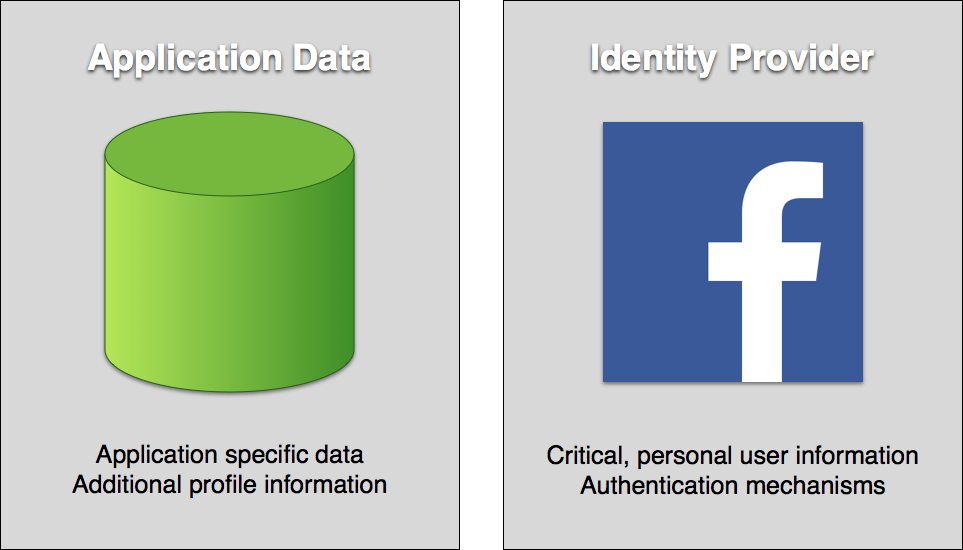
\includegraphics[width=9cm]{content/principle-demonstration/images/applicationdata-vs-identityprovider.png}
	\caption{Separierung der Applikations- und Identitätsinformationen}
	\label{fig:applicationdata-vs-identityprovider}
\end{figure}

In der Abbildung \ref{fig:applicationdata-vs-identityprovider} ist zudem ersichtlich dass ein \emph{Identity Provider} meist auch den Mechanismus zur effektiven Authentisierung des Benutzers bereitstellt. Viele Anbieter setzen hier auf den de facto Standard \emph{OAuth} \cite{oauth} oder verwenden eigene Implementationen.


\subsection*{Geplante Umsetzung}

Für die Beispielapplikation \emph{Roomies} hat das Projektteam geplant, Facebook als hauptsächlichen und einzigen \emph{Identity Provider} zu einzusetzen. Dabei soll das offizielle \emph{Facebook Login for Web} \cite{facebooklogin} \gls{SDK} eingesetzt werden.

Innerhalb der Beispielapplikation soll lediglich die Facebook ID sowie der Name des Benutzers persistent gespeichert werden. Alle anderen Informationen sollen bei Facebook verbleiben resp. gar nicht erst auf diese zugegriffen werden.


\subsection*{Konkrete Umsetzung}

Für die tatsächliche Anbindung des \emph{Facebook Login for Web} \cite{facebooklogin} \gls{SDK}'s wurde wie im Abschnitt \ref{sec:sad-layers} ``\nameref{sec:sad-layers}'' des Kapitels ``\nameref{sec:sad}'' beschrieben durch die quelloffene Bibliothek \emph{Passport} \cite{Passportjs} umgesetzt.

Die verfügbare \emph{Authentication Strategy} für Facebook \cite{passport-facebook} ermöglicht das einfache Einbinden der Facebook Anmeldemechanismen in jede \emph{Express.js} Applikation.

Zudem werden wie geplant lediglich Facebook ID und Name eines Benutzers in der Applikationsdatenbank abgelegt. Über eine öffentlich zugängliche \gls{URL} \cite{facebook-profilepicture} wird zusätzlich das aktuelle Profilbild des Benutzers in der Menüleiste von \emph{Roomies} angezeigt, jedoch nicht innerhalb der Applikation zwischengespeichert.

\begin{figure}[H]
	\centering
	
\includegraphics[width=10cm]{content/principle-demonstration/images/roomies-navigation-loggedin.png}
	\caption{Facebook Profilbild des angemeldeten Benutzers der Menüleiste der Beispielapplikation \emph{Roomies}}
	\label{fig:facebook-profilepicture-roomies}
\end{figure}


\subsection*{Diskussion}

Lange Zeit hielten sich hartnäckige Vorbehalte gegenüber der Verwendung von Facebook o.Ä. Konten für die Anmeldung bei Diensten Dritter. Immer mehr lässt sich jedoch eine gewisse Akzeptanz bei den Benutzern im Internet feststellen. Verbesserte und klarer deklarierte Möglichkeiten zur Anpassung der Zugriffseinstellungen auf hinterlegte Informationen \cite{facebook-authdialog} haben hier definitiv ihren Teil beigetragen.

Für den Dienstanbieter bringt die Verwendung eines externen \emph{Identity Providers} grosse Vorteile mit sich: Er kann sich auf seine Kernkompetenzen konzentrieren, insbesondere wenn zur Integration umfangreiche Frameworks wie eben \emph{Passport} verwendet werden können.

So ist es, eine entsprechende Architektur vorausgesetzt, möglich, ohne grössere Zusatzaufwände weitere \emph{Provider} anzubinden. Im Falle der vorliegenden Beispielapplikation ist die Integration von \emph{Twitter}, um nur einen \emph{Identity Provider} zu nennen, genau so einfach umsetzbar, wie die Implementation einer komplett eigenständigen Lösung.

Welche Möglichkeiten zur Anmeldung bei einem Dienst angeboten werden sollen ist wie so oft abhängig von vielen Faktoren. Für kritische Applikationen wie eBanking-Suiten mag es Heute lächerlich klingen, sich via Facebook-Konto anzumelden. Die grosse Verbreitung von PayPal \cite{paypal} als zentralen Anbieter von Geldtransaktionsdiensten zeigt aber, dass selbst hier mit entsprechenden Sicherheitsmassnahmen viel Skepsis wett gemacht werden kann.

Wird eine weniger kritische Applikation konzipiert und ist mit Akzeptanz in der potentiellen Nutzergruppe zu rechnen, empfiehlt das Projektteam uneingeschränkt die von \emph{TP4 Separate user identity, sign-up and self-care from product dependencies} vorgeschlagene Teilung von Applikations- und Identitätsinformationen resp. Authentifizierungsmechanismen.

%\section{TP7 Apply the Web instead of working around}
\label{sec:principle-tp7-apply-the-web}

Der moderne Internetbrowser kapselt eine Vielzahl von leistungsfähigen Funktionen des jeweiligen Hostrechner in ein für den Software Entwickler leicht zu verwendendes Interface. Dazu gehört die Integration von systemnahen Komponenten wie \gls{GPU}'s \cite{webgl} genauso wie die Möglichkeit, gleichzeitig mehrere Fenster oder Tabs für die selbe oder verschiedenen Applikationen resp. Internetseite offen zu halten.

Das Hin- und Herspringen zwischen besuchten Seiten mittels Vorwärts- und Zurück-Schaltflächen gehört seit Beginn der Webära zum festen Bestandteil der User Experience im Internet.

In der Vergangenheit gehörten wiederkehrende Umsetzungen von Funktionen wie der Validierung von Formularinhalten zu lästigen, aber nötigen Ärgernissen. Mit der Einführung der neusten Revision 5 des HTML Standards können gerade solche Aufgaben bequem dem Browser \cite{HTML5Forms} überlassen werden

Mit der immer mächtiger werdenden Formatierungssprache CSS und dessen neuster Version 3 sind heute gestalterische Effekte möglich, welche bis vor Kurzem nur mittels umständlicher Einbindung von Grafikdateien (Stichwort Schlagschatten \cite{css-box-shadow} oder Farbverlauf \cite{css-gradient}) möglich waren.

Mit der Richtlinie \emph{TP7} hält Stefan Tilkov Software Entwickler dazu an, die Werkzeuge welche vom Internetbrowser angeboten werden, gewinnbringend zu nutzen.


\subsection*{Geplante Umsetzung}

In der Beispielapplikation sollen gezielt HTML 5 Features verwendet werden:

\begin{itemize}
	\item Semantisch korrekte Tags (\emph{<header>}, \emph{<section>} etc.) \cite{SemanticHTML}
	\item Formularvalidierung \cite{HTML5Forms}
\end{itemize}

Das entstehende, semantisch korrekte HTML Markup soll mit CSS 3 gestaltet werden. Neue Möglichkeiten zur grafischen Darstellung sollen ausgenutzt werden. Die Verwendung von \emph{Media Queries} \cite{css-mediaquery} soll die  Darstellung auf verschiedenen Bildschirmen (Desktops, Tablets, Smartphones usw.) optimieren und vereinfachen.

Bei der Entwicklung der Front- als auch Backend-Komponente muss zwingend darauf geachtet werden, dass die Verwendung der Browser-Funktionen \emph{Vorwärts}, \emph{Zurück} und \emph{Aktualisieren} zu keinem ungewünschten resp. unerwarteten Verhalten führen.


\subsection*{Konkrete Umsetzung}

\subsubsection*{HTML Markup}

Das gerenderte HTML Markup verwendet wie geplant vom HTML 5 Standard eingeführte Funktionen. Quellcode \ref{lst:roomiesMenuHtml} zeigt die Verwendung des \emph{<header>} sowie \emph{<nav>} Tags zur Beschreibung des Applikationsmenüs der Beispielapplikation.

\begin{lstlisting}[language=HTML, caption={Ausschnitt des gerenderten HTML Markups der Menüleiste \emph{roomies}}, label={lst:roomiesMenuHtml}]
<header id="menu">
	<div class="fixed-navigation">
		<nav class="navigation" role="navigation">
			<div class="title-area">
				<a href="/" class="banner" title="Roomies"><h1>Roomies</h1></a>
			</div>
			<section class="nav-section">
				<ul class="left">
						<li>
							<a href="/community/ba-team/tasks" title="Aufgaben">
								<i class="icon-tasks icon-large"></i>
								<span class="item-label"> Aufgaben</span>
							</a>
						</li>
						<!-- ... more items -->
				</ul>
				<!-- ... displaying the facebook profile picture -->
			</section>
		</nav>
	</div>
</header>
\end{lstlisting}

Weiter wurde für das \emph{Fällig bis}-Feld auf der Ansicht \emph{Aufgabe bearbeiten} ein Textfeld vom Typ \emph{date} verwendet. Gerade auf einem Mobile Browser wie \emph{Safari für iPhone} kommt diese Implementation voll zum tragen.

\begin{figure}[H]
	\centering
	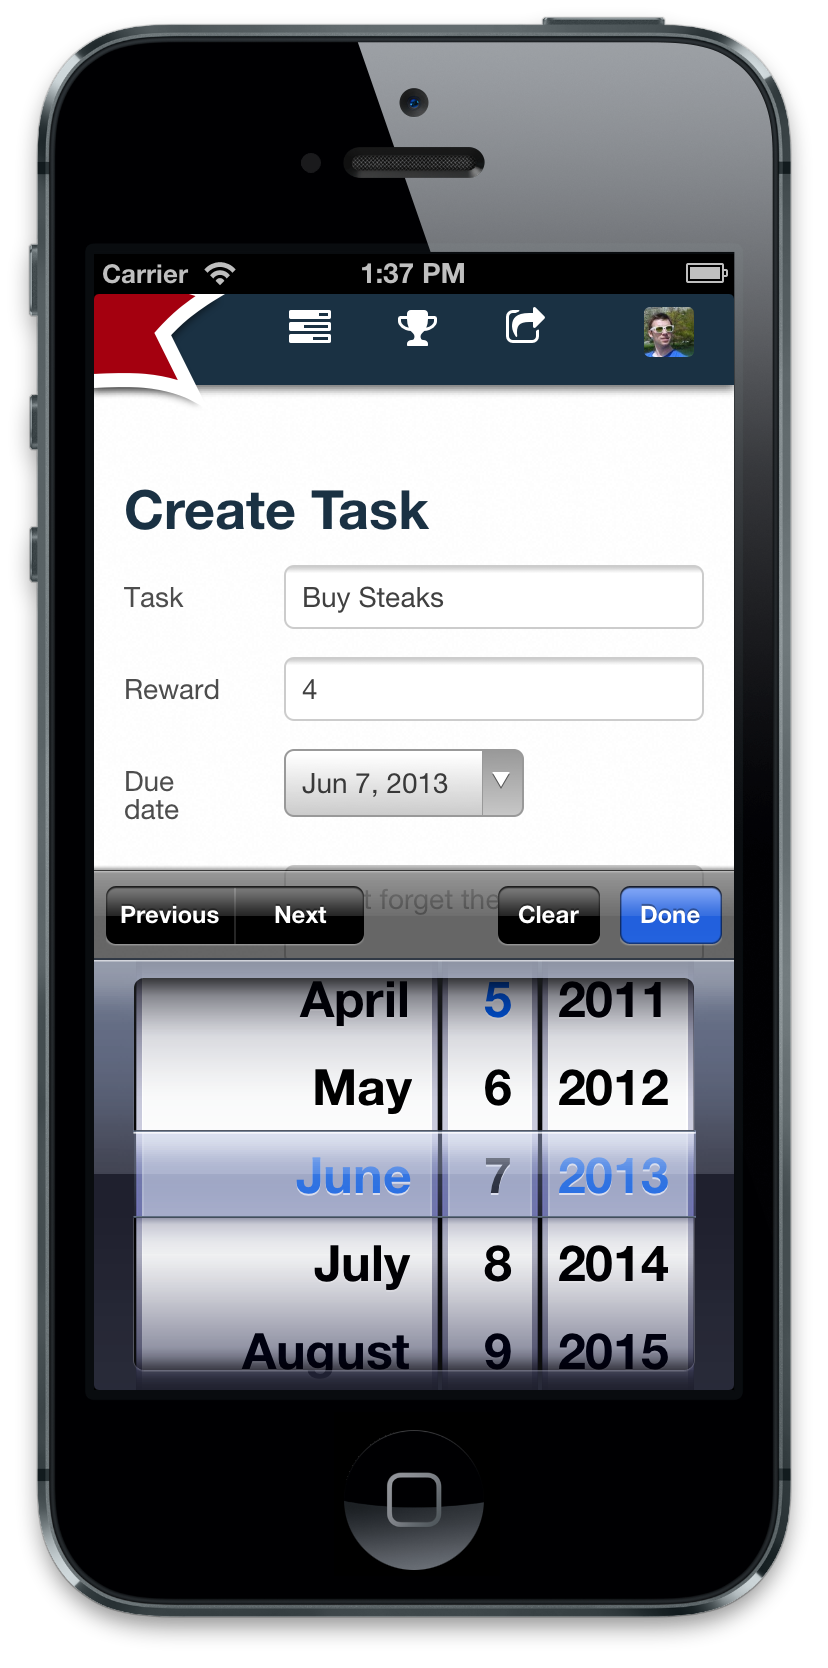
\includegraphics[width=6cm]{content/principle-demonstration/images/iossafari-datepicker.png}
	\caption{Datumsauswahl für ein Textfeld vom Typ \emph{date} in \emph{Safari für iPhone}}
	\label{fig:iossafari-datepicker}
\end{figure}


\subsubsection*{CSS}

Der erstellte CSS Quellcode macht ausführlichen Gebrauch der neusten CSS 3 Features. So wird für die Darstellung von visuellen Effekten oft auf \emph{box-shadow} oder halbtransparente Farben zurückgegriffen.

Verschiedene Internetbrowser interpretieren CSS Formatierungsbefehle teilweise immer noch sehr unterschiedlich. Um diesem Problem beizukommen wurde die SASS Funktionsbibliothek \emph{Bourbon} \cite{bourbon} eingesetzt. Verschiedene Mixins ermöglichen mit der Verwendung des SASS Präprozessors \cite{SASS} das Generieren von crossbrowser-kompatiblem CSS Quelltext.

\begin{lstlisting}[language=JavaScript, firstnumber=4, caption={Einbindung des \emph{@border-radius} Mixins von \emph{Bourbon} \cite{RoomiesSassBorderRadiusMixin}}, label={lst:roomiesSassBorderRadiusMixin}]
.button {
	@include button($button-color-bg);
	@include border-radius(8px);
	margin-top: 1px;
\end{lstlisting}

Im Bereich \emph{Responsive Design} wurde ebenfalls keine Lösung von Grund auf selber entwickelt. Unter Zuhilfenahme der \emph{Foundation} SASS Bibliothek \cite{Foundation} wurde auf einfache Art und Weise ein flexibles User Interface Layout entworfen, welches dynamisch auf die verschiedenen Bildschirmgrössen reagieren kann.

\begin{figure}[H]
	\centering
	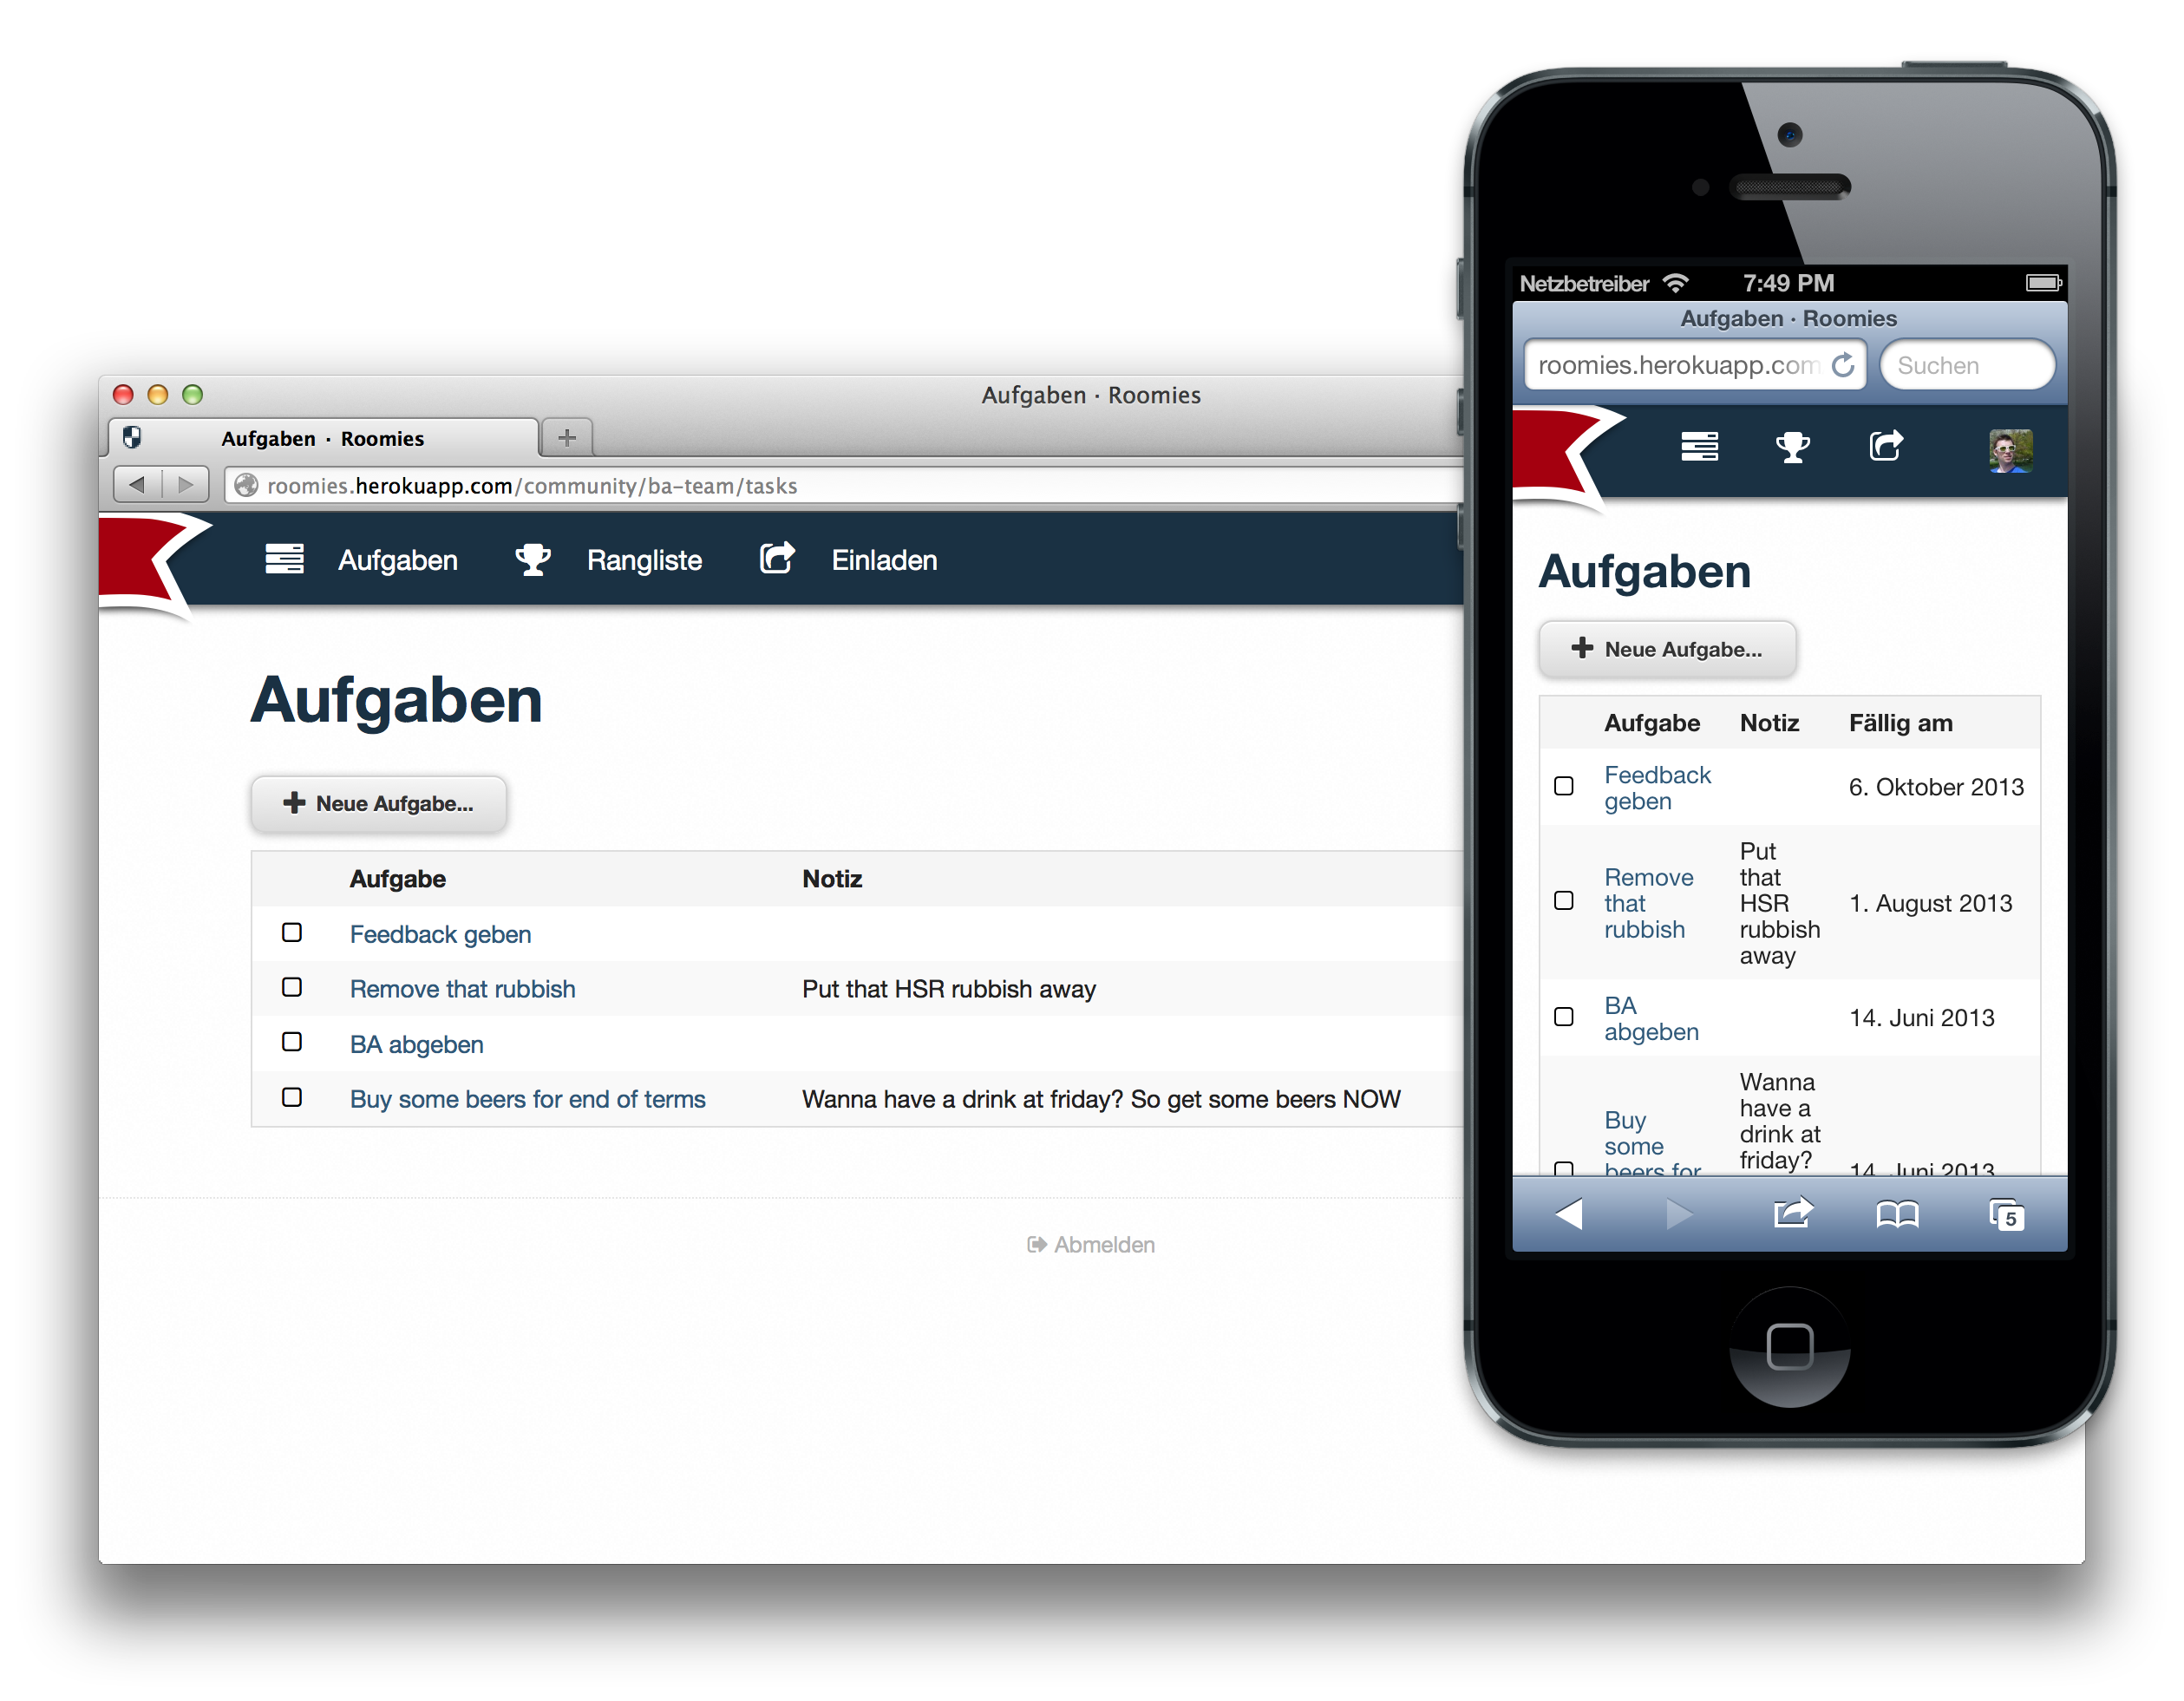
\includegraphics[width=9cm]{content/principle-demonstration/images/responsive-screenshots.png}
	\caption{Media Queries ermöglichen dynamische Anpassung des Layouts entsprechend der verfügbaren Bildschirmgrösse}
	\label{fig:responsive-screenshots}
\end{figure}


\subsubsection*{Navigation mittels Browserfunktionen}

Wie geplant konnte ein einheitliches Navigationsverhalten implementiert werden. Der Benutzer kann sowohl Browsersteuerelemente als auch applikationsinterne Links zur Navigation verwenden, ohne ein unerwartetes Verhalten zu provozieren.

Ausführlichere Informationen zu dieser Thematik sind Abschnitt \ref{sec:principle-rp10-browser-controls} ``\nameref{sec:principle-rp10-browser-controls}'' enthalten.


\subsubsection*{iOS Webapp Kompatibilität}

Zusätzlich zu den geplanten Features wurde die von Apple definierte Spezifikation für \emph{Web Applications} \cite{SafariWebApp} in \emph{Roomies} integriert. Entsprechende Metatags im \emph{<head>}-Bereich des HTML Markups ermöglichen eine bessere Integration der Applikation in die iOS Umgebung. Dazu gehört u.A. ein eigenes Bookmark-Symbol für den iOS Homescreen (siehe Abbildung \ref{fig:webapp-homescreen-icon}) als auch angepasste Ladebildschirme während dem \emph{Aufstarten} der Applikation.

\begin{figure}[H]
	\centering
	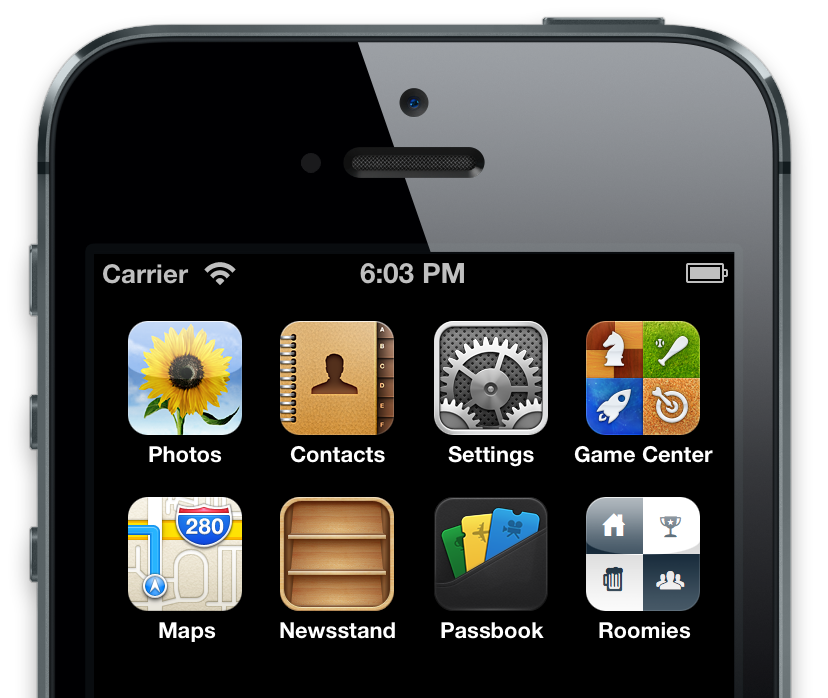
\includegraphics[width=6cm]{content/principle-demonstration/images/ios-webapp-homescreenicon.png}
	\caption{\emph{Roomies} als Webapp auf dem iPhone Homescreen}
	\label{fig:webapp-homescreen-icon}
\end{figure}


\subsection*{Diskussion}

Mächtigere Browser ermöglichen die Ausführung immer ausgefeilterer Internetapplikationen. Umfangreiche Browser API's ersparen die Implementierung eigener Überprüfungsmechanismen für Benutzereingaben oder erleichtern die Gestaltung ansprechender User Interfaces.

In Zukunft wird es zudem vermehrt Möglichkeiten geben, wie vermeintlich schwerfällige Webapplikationen in die Betriebssystemumgebung von Smartphones integriert werden können. Diesbezüglich darf man sehr auf Firefox OS gespannt sein, welches den Ansatz von Apples Webapps auf die Spitze treiben wird \cite{FirefoxOSWebApp}.

Leider scheitern die neuen Standards, welche de facto offiziell noch keine sind, momentan oft an den herstellerspezifischen Implementierungen. So erscheint auf dem iPhone ein benutzerfreundlicher Helfer für die Auswahl eines Datums, in \emph{Mozilla Firefox} \cite{CanIUseDateInput} wird das Datumseingabefeld weiterhin als einfaches Textfeld angezeigt. Für eine Webapplikation hat dies zur Folge, dass im Client weiterhin Logik für die Überprüfung von Benutzereingaben implementiert werden muss. Unter dem Aspekt von Sicherheitsmassnahmen mag die grundsätzlich logisch erscheinen, bedeutet dies aber trotzdem eine erhöhten Aufwand im Entwicklungsprozess.

Viele der neuen Browserfeatures können bereits heute angewendet werden. Durch die mangelnde Standardisierung unter den verschiedenen Browserherstellern ergibt sich für das Projektteam jedoch ein eher durchzogener Eindruck der Situation auf diesem Gebiet der Webstandards.

Aus diesem Grund ermutigt das Projektteam zwar zur Verwendung neuester Funktionalitäten, ermahnt jedoch immer eine Fallbacklösung bereitzuhalten, sollte ein Feature auf einem Browser nicht verfügbar sein.

\section{TP8 Automate everything or you will be hurt}
\label{sec:principle-tp8-automate-everything}

\emph{TP8} greift einen allgemein gültigen Vorsatz aus dem Software Engineering auf: Mit ``\emph{\gls{DRY}}'' wird zum einen sich wiederholender Quellcode minimiert, zum anderen werden auch wiederkehrende Routineaufgaben automatisiert.

Entwickelt man den ``\emph{\gls{DRY}}''-Ansatz weiter, so landet man unweigerlich bei der Verwendung von automatisierten Tests und Deployments mittels Continuous Integration Systemen.

\subsection*{Geplante Umsetzung}
Gemäss Tabelle \ref{fig:how-to-show-principles-matrix} ``\nameref{fig:how-to-show-principles-matrix}'' im Kapitel ``\nameref{sec:analyse-der-aufgabenstellung}'' soll \emph{TP8} durch die Verwendung verschiedener unterstützender Tools umgesetzt und demonstriert werden.

Tabelle \ref{fig:automated-tasks-planned} zeigt eine Auflistung der zu automatisierenden Aufgaben:

\begin{table}[H]
\tablestyle
\tablealtcolored
\begin{tabularx}{\textwidth}{l X}
\tableheadcolor
	\tablehead ID &
	\tablehead Aufgabe
	\tabularnewline
\tablebody
	\textit{TP8.1} & Starten der Beispielapplikation\tabularnewline
	\textit{TP8.2} & Ausführung der Unit Tests\tabularnewline
	\textit{TP8.3} & Formale Überprüfung des Quellcodes\tabularnewline
	\textit{TP8.4} & Umwandlung von SASS zu CSS Stylesheets\tabularnewline
	\textit{TP8.5} & Erstellung von Quellcode Dokumentation\tabularnewline
\tableend
\end{tabularx}
\caption{Automatisierte Aufgaben (geplant)}
\label{fig:automated-tasks-planned}
\end{table}


\subsection*{Konkrete Umsetzung}
Neben den oben erwähnten Aufgaben wurden in der konkreten Implementation des Projektes weitere Tasks erfolgreich automatisiert:

\begin{table}[H]
\tablestyle
\tablealtcolored
\begin{tabularx}{\textwidth}{l X l}
\tableheadcolor
	\tablehead ID &
	\tablehead Aufgabe &
	\tablehead \gls{CLI} Befehl
	\tabularnewline
\tablebody
	\textit{TP8.1} & Starten der Beispielapplikation & \emph{npm start}\tabularnewline
	\textit{TP8.2} & Ausführung der Unit Tests & \emph{make test}\tabularnewline
	\textit{TP8.3} & Qualitative Überprüfung des Quellcodes (Code Style Guidelines) & \emph{make lint}\tabularnewline
	\textit{TP8.4} & Umwandlung von SASS zu CSS Stylesheets & \emph{make precompile-sass}\tabularnewline
	\textit{TP8.5} & Erstellung von Quellcode Dokumentation & \emph{make docs}\tabularnewline
	\textit{TP8.6} & Vorbereitung von View Templates & \emph{make precompile-templates}\tabularnewline
	\textit{TP8.7} & Veröffentlichung von Dokumentation (dieses Dokument, aber auch Quellcode Dokumentation), Testergebnissen und Test Code Coverage Reports & Travis CI\tabularnewline
	\textit{TP8.8} & Umwandlung des LaTeX Quellcodes zur finalen PDF Dokumentation (Dokumentations Repository) & \emph{make}\tabularnewline
	\textit{TP8.9} & Installation der Beispielapplikation & \emph{./install.sh}\tabularnewline
\tableend
\end{tabularx}
\caption{Automatisierte Aufgaben (umgesetzt)}
\label{fig:automated-tasks-concrete}
\end{table}

Als Kernkomponente für die Automatisierung der Aufgaben in Tabelle \ref{fig:automated-tasks-concrete} wird ein \emph{Makefile} (\cite{RoomiesMakefile} und \cite{ThesisMakefile}) verwendet. Dieses wird von \emph{GNU Make} \cite{make} interpretiert und ermöglicht so das Ausführen verschiedenster Operationen.

Der Quelltext \ref{lst:makefileDocs} zeigt exemplarisch die Befehlsdefinition für die Erstellung der Quellcode Dokumentation mittels \emph{Natural Docs} \cite{NaturalDocs}.

\begin{lstlisting}[language=Bash, firstnumber=99, caption={Ausschnitt Makefile: Code Dokumentation erstellen} \cite{RoomiesMakefile}, label=lst:makefileDocs]
docs:
	-mkdir ./docs
	@NaturalDocs -i ./src -o HTML ./docs -p ./.naturaldocs -xi ./src/server/public -s Default style
\end{lstlisting}

Durch den einfache Kommandozeilenbefehl \emph{make docs} wird der in \ref{lst:makefileDocs} definierte Befehl ausgeführt.


\subsection*{Continuous Integration}

Die in Tabelle \ref{fig:automated-tasks-concrete} vorgestellten Aufgaben \emph{TP8.2} bis \emph{8.8} werden sowohl lokal auf dem Entwicklerrechner als auch auf dem Continuous Integration System ausgeführt.

Entsprechend der Definition in Kapitel \ref{sec:qualitymanagement} ``\nameref{sec:qualitymanagement}'' wird hierzu die Open Source Plattform Travis CI \cite{TravisCI} verwendet. Der Quelltext \ref{lst:roomiesTravisYML} zeigt einen Ausschnitt der Datei \emph{.travis.yml} \cite{RoomiesTravisYML}. Diese steuert den Build auf Travis CI.

\begin{lstlisting}[language=XML, firstnumber=5, caption={Ausschnit aus .travis.yml \cite{RoomiesTravisYML}}, label=lst:roomiesTravisYML]
before_install:
    - ./travis/before_install.sh

after_success:
    - ./travis/after_success.sh

language: node_js
node_js:
  - 0.8

script: "make docs test-coveralls lint"
\end{lstlisting}

\subsection*{Diskussion}
Muss eine Aufgabe zweimal ausgeführt werden, sollte dies als Rechtfertigung zur Automatisierung einer solchen Arbeit bereits genügen. Dies trifft umso mehr zu, wenn mehrere Entwickler am Entwicklungsprozess beteiligt sind.

Die Praxis zeigt, dass Zeitersparnis und Effektivitätssteigerung die positiven Folgen der Automatisierung von Routineaufgaben sind. Wird die Ausführung der Unit Tests erleichtert, lässt sich zudem die Akzeptanz eines Test Driven Development Prozesses erhöhen.

Das Projektteam war positiv davon überrascht, was sich mit frei zugänglichen Continuous Integration Lösungen wie Travis CI \cite{TravisCI} umsetzen lässt. Von der Generierung von Dokumentationen bis hin zur regelmässigen Ausführung von Unit Tests lassen sich ohne grossen Aufwand unbeliebte Aufgaben problemlos automatisieren und auslagern.

Das Credo ``Don't repeat yourself'' ist somit ganz klar Trumpf und so wird auch die Richtlinie \emph{TP8 Automate everything or you will be hurt} vom Projektteam unterstützt.

%\section{Abschliessende Bewertung}

todo